\section{Input}

\textbf{Input Devices}

Fitt's law for performance evaluation of input devices, but how to distinguish in functionality and specific metric? Answer is systematization. 
In general input devices enable to engange in dialogue with a computer or a machine. This dialogue is not in natural language. 
Dialogue is between fundamentally dissimilar agents-both in perception and processing. \medskip

"It's a transducer from the physical properties of the world into logical values of the application." \medskip

\textbf{Fitts' Law in 2D}

\begin{center}
	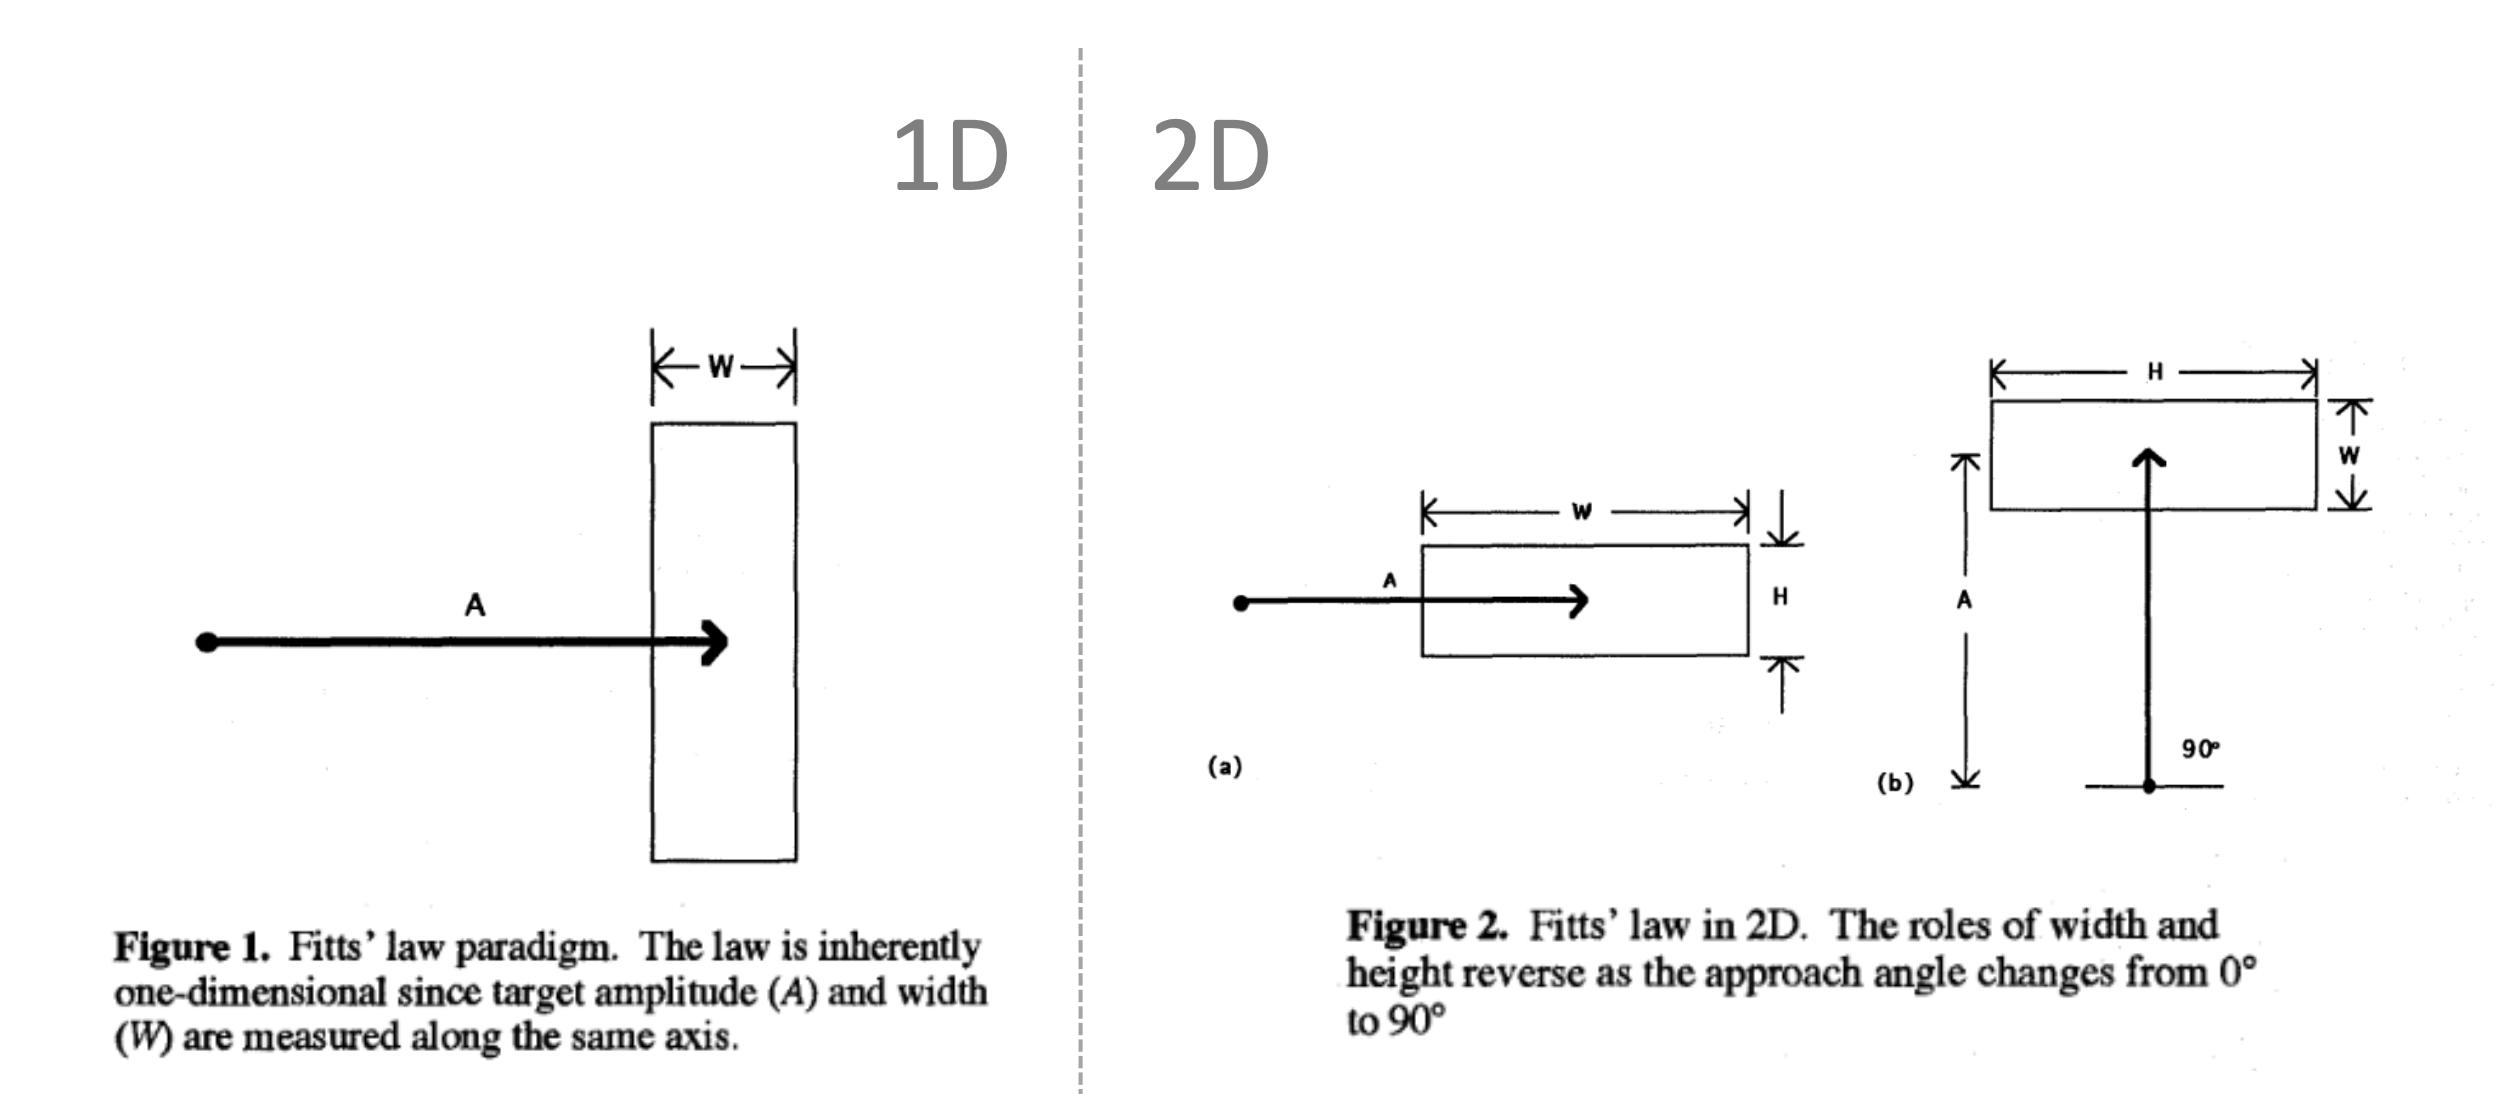
\includegraphics[width=\linewidth]{fitts_law_2d.png}
\end{center}

\begin{center}
	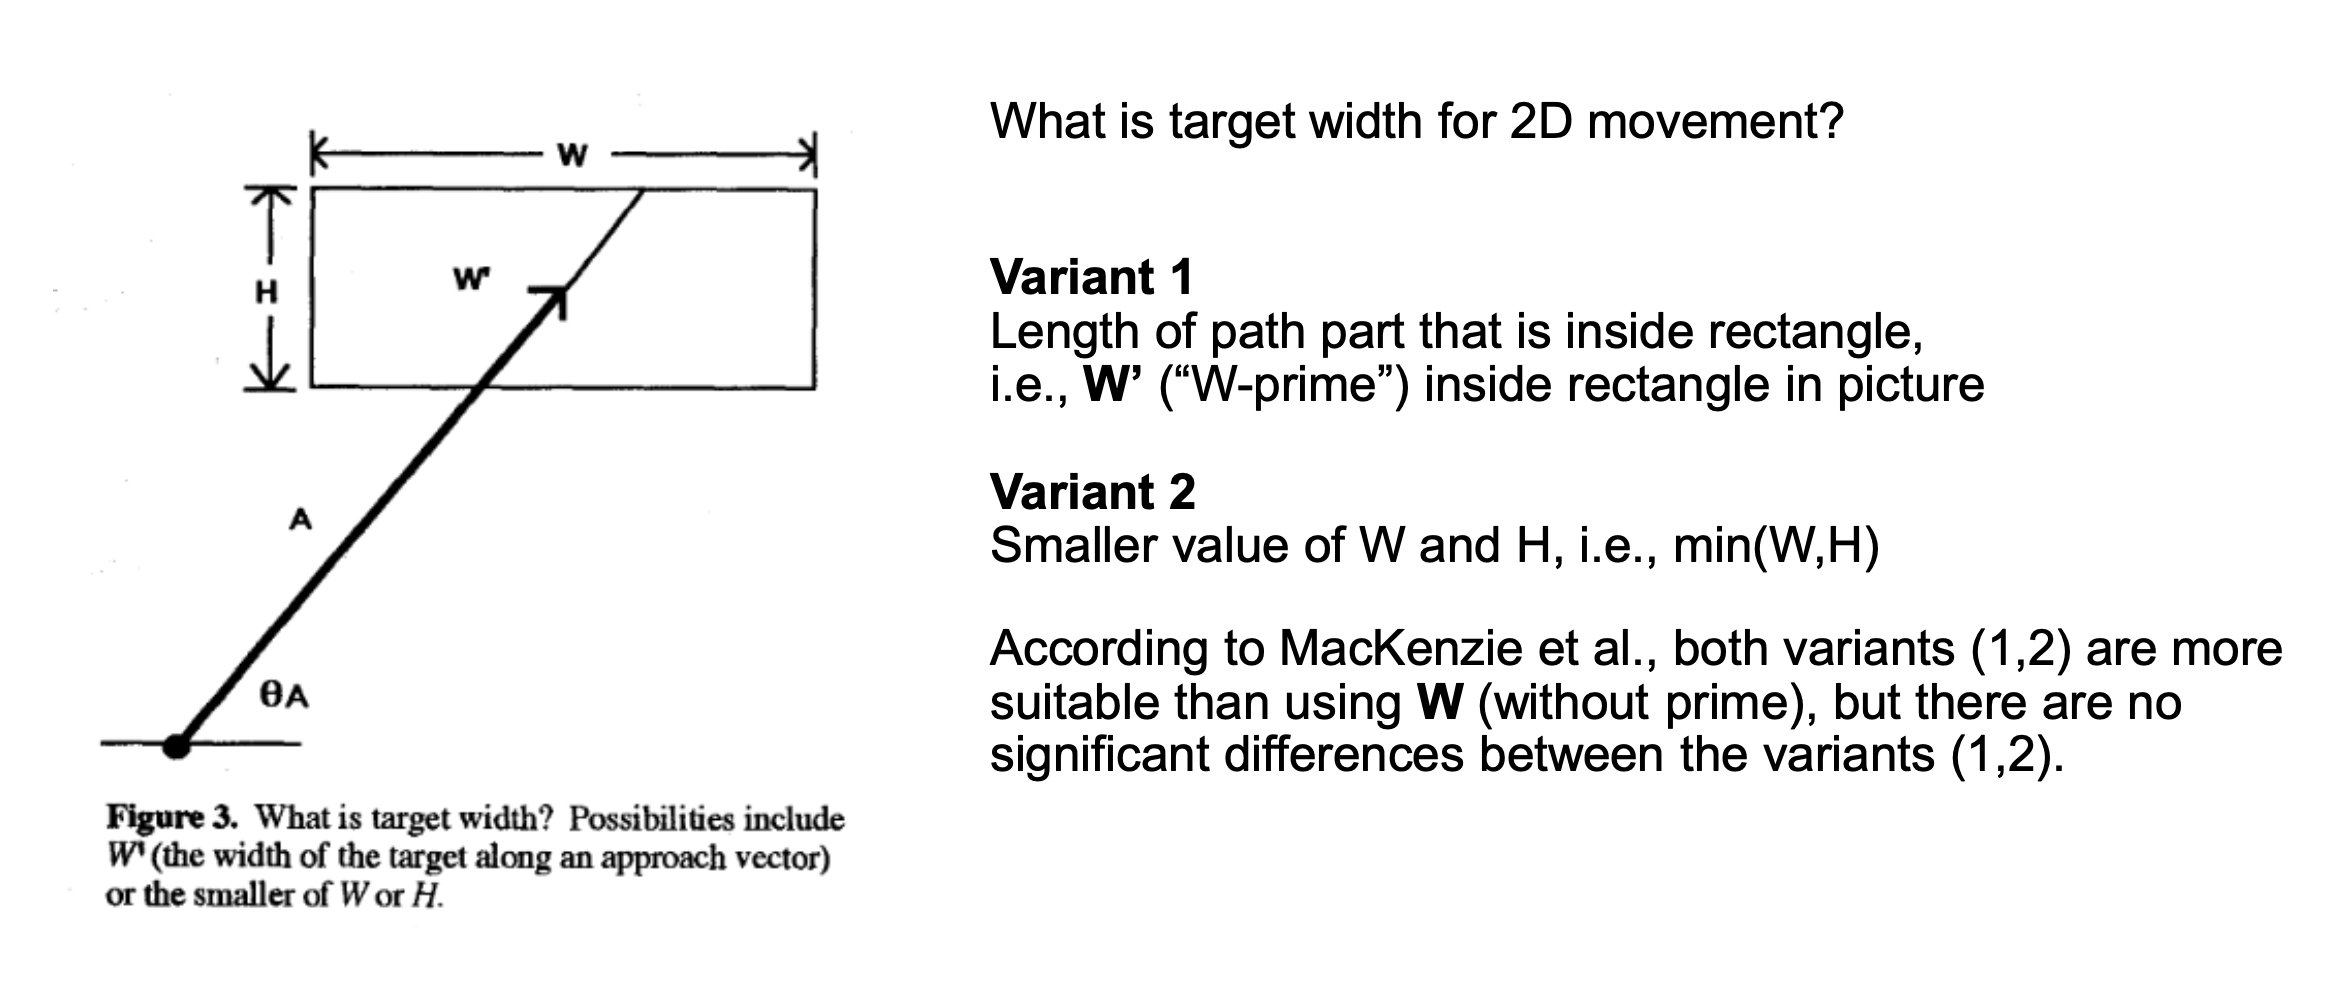
\includegraphics[width=\linewidth]{fitts_law_2d_2.png}
\end{center}

\textbf{Properties} \smallskip

\textit{Direct / indirect input} \smallskip

\begin{itemize}[itemsep=-5pt, topsep=0pt, leftmargin=*]
	\item Direct: Touchscreen, "grasping" virtual 3d objects
	\item Indirect: Mouse movement translated to cursor position (virtual cursor can directly/indirectly manipulate virtual content)
\end{itemize}

\textit{Absolute / relative} \smallskip

\begin{itemize}[itemsep=-5pt, topsep=0pt, leftmargin=*]
	\item Absolute: Position of input mapped to position of output (e.g. drawing tablet)
	\item Relative: Change of input position mapped to change of output position (e.g. mouse)
\end{itemize}


\textit{Position control / rate control} \smallskip


\begin{itemize}[itemsep=-5pt, topsep=0pt, leftmargin=*]
	\item Manipulate position of something (e.g. mouse cursor) versus its velocity (e.g. thumbstick)
\end{itemize} \medskip

\textit{Degrees of freedom} \smallskip

\begin{itemize}[itemsep=-5pt, topsep=0pt, leftmargin=*]
	\item Examples: only 2D position along surface (2 DoF), 3D position and rotatoin in mid-air (6 DoF), or other combination (3D position + rotation around one axis : 4 DoF)
\end{itemize} \medskip

\textit{Isotonic / elastic / isometric} \smallskip

\begin{itemize}[itemsep=-5pt, topsep=0pt, leftmargin=*]
	\item Movable (isotonic e.g. mouse) vs. movable but goes back to neutral position (elastic, e.g. joystick) vs. immovable (isometric, sense force only e.g. lenovo red dot)
\end{itemize} \medskip

\textbf{Performance/Bandwidth} \smallskip

The performance depends on the human (bandwidth of muscle groups connected to input device), the device (effective bandwidth of input device) 
and application (precision requirements of the task). \medskip

\textbf{Effectiveness} \smallskip

\begin{multicols}{2}
    \begin{itemize}[itemsep=-5pt, topsep=0pt, leftmargin=*]
	\item Pointing speed
	\item Pointing precision
	\item errors
	\item Time to learn
	\item Time to grasp device
	\item User preference
	\item Desk footprint
	\item Cost
	\end{itemize}
\end{multicols}


\textbf{Design Space by Card et al} \smallskip

Input device as six-tuple: (M, In, S, R, Out, W) \smallskip

\begin{multicols}{2}
    \begin{itemize}[itemsep=-5pt, topsep=0pt, leftmargin=*]
	\item M: Manipulation operator
	\item In: Input Domain
	\item S: Current state of device
	\item R: (Resolution) Mapping from input domain to output domain
	\item Out: Output domain
	\item W: Additional aspects of ow device works (input lag etc.)
	\end{itemize}
\end{multicols}


\begin{center}
	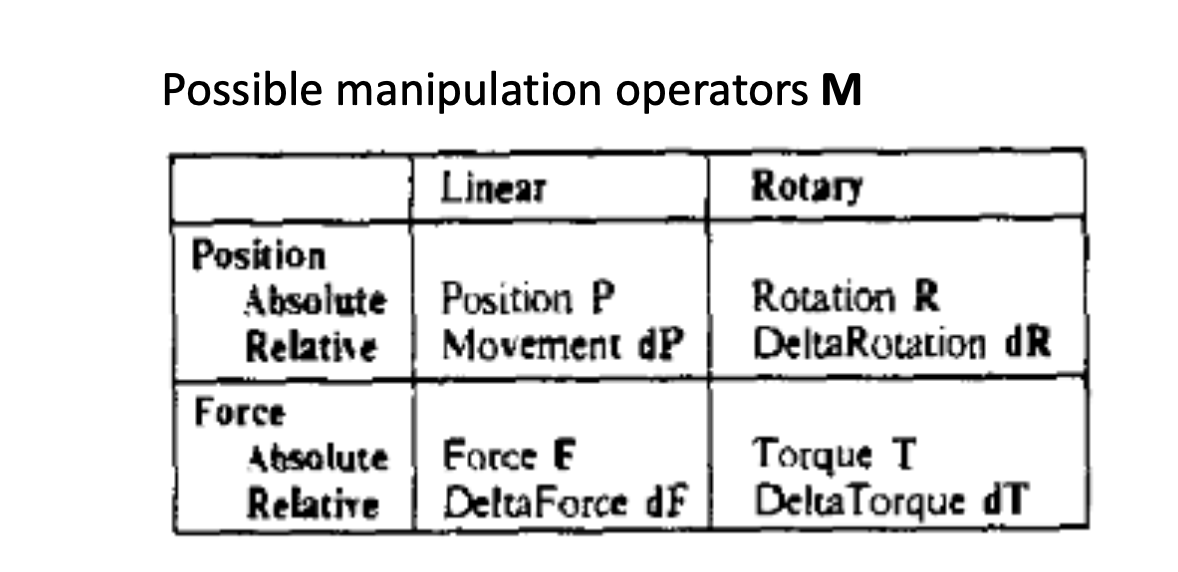
\includegraphics[width=\linewidth]{manipulation_operators.png}
\end{center}

\textbf{Composition operators} \smallskip

\begin{itemize}[itemsep=-5pt, topsep=0pt, leftmargin=*]
	\item Merge composition: e.g. sensed X-Y movement of mouse merged into 2D input
	\item Layout composition: Seperate independent inputs on a device (e.g. independent buttons or wheels on mouse)
	\item Connect composition: Output of one device/sensor mapped into input of another (e.g. physical mouse is input for virtual screen cursor). In this context virtual cursors count also as input devices. 
\end{itemize}

\textbf{Card's Graphical representation} \smallskip


\begin{center}
	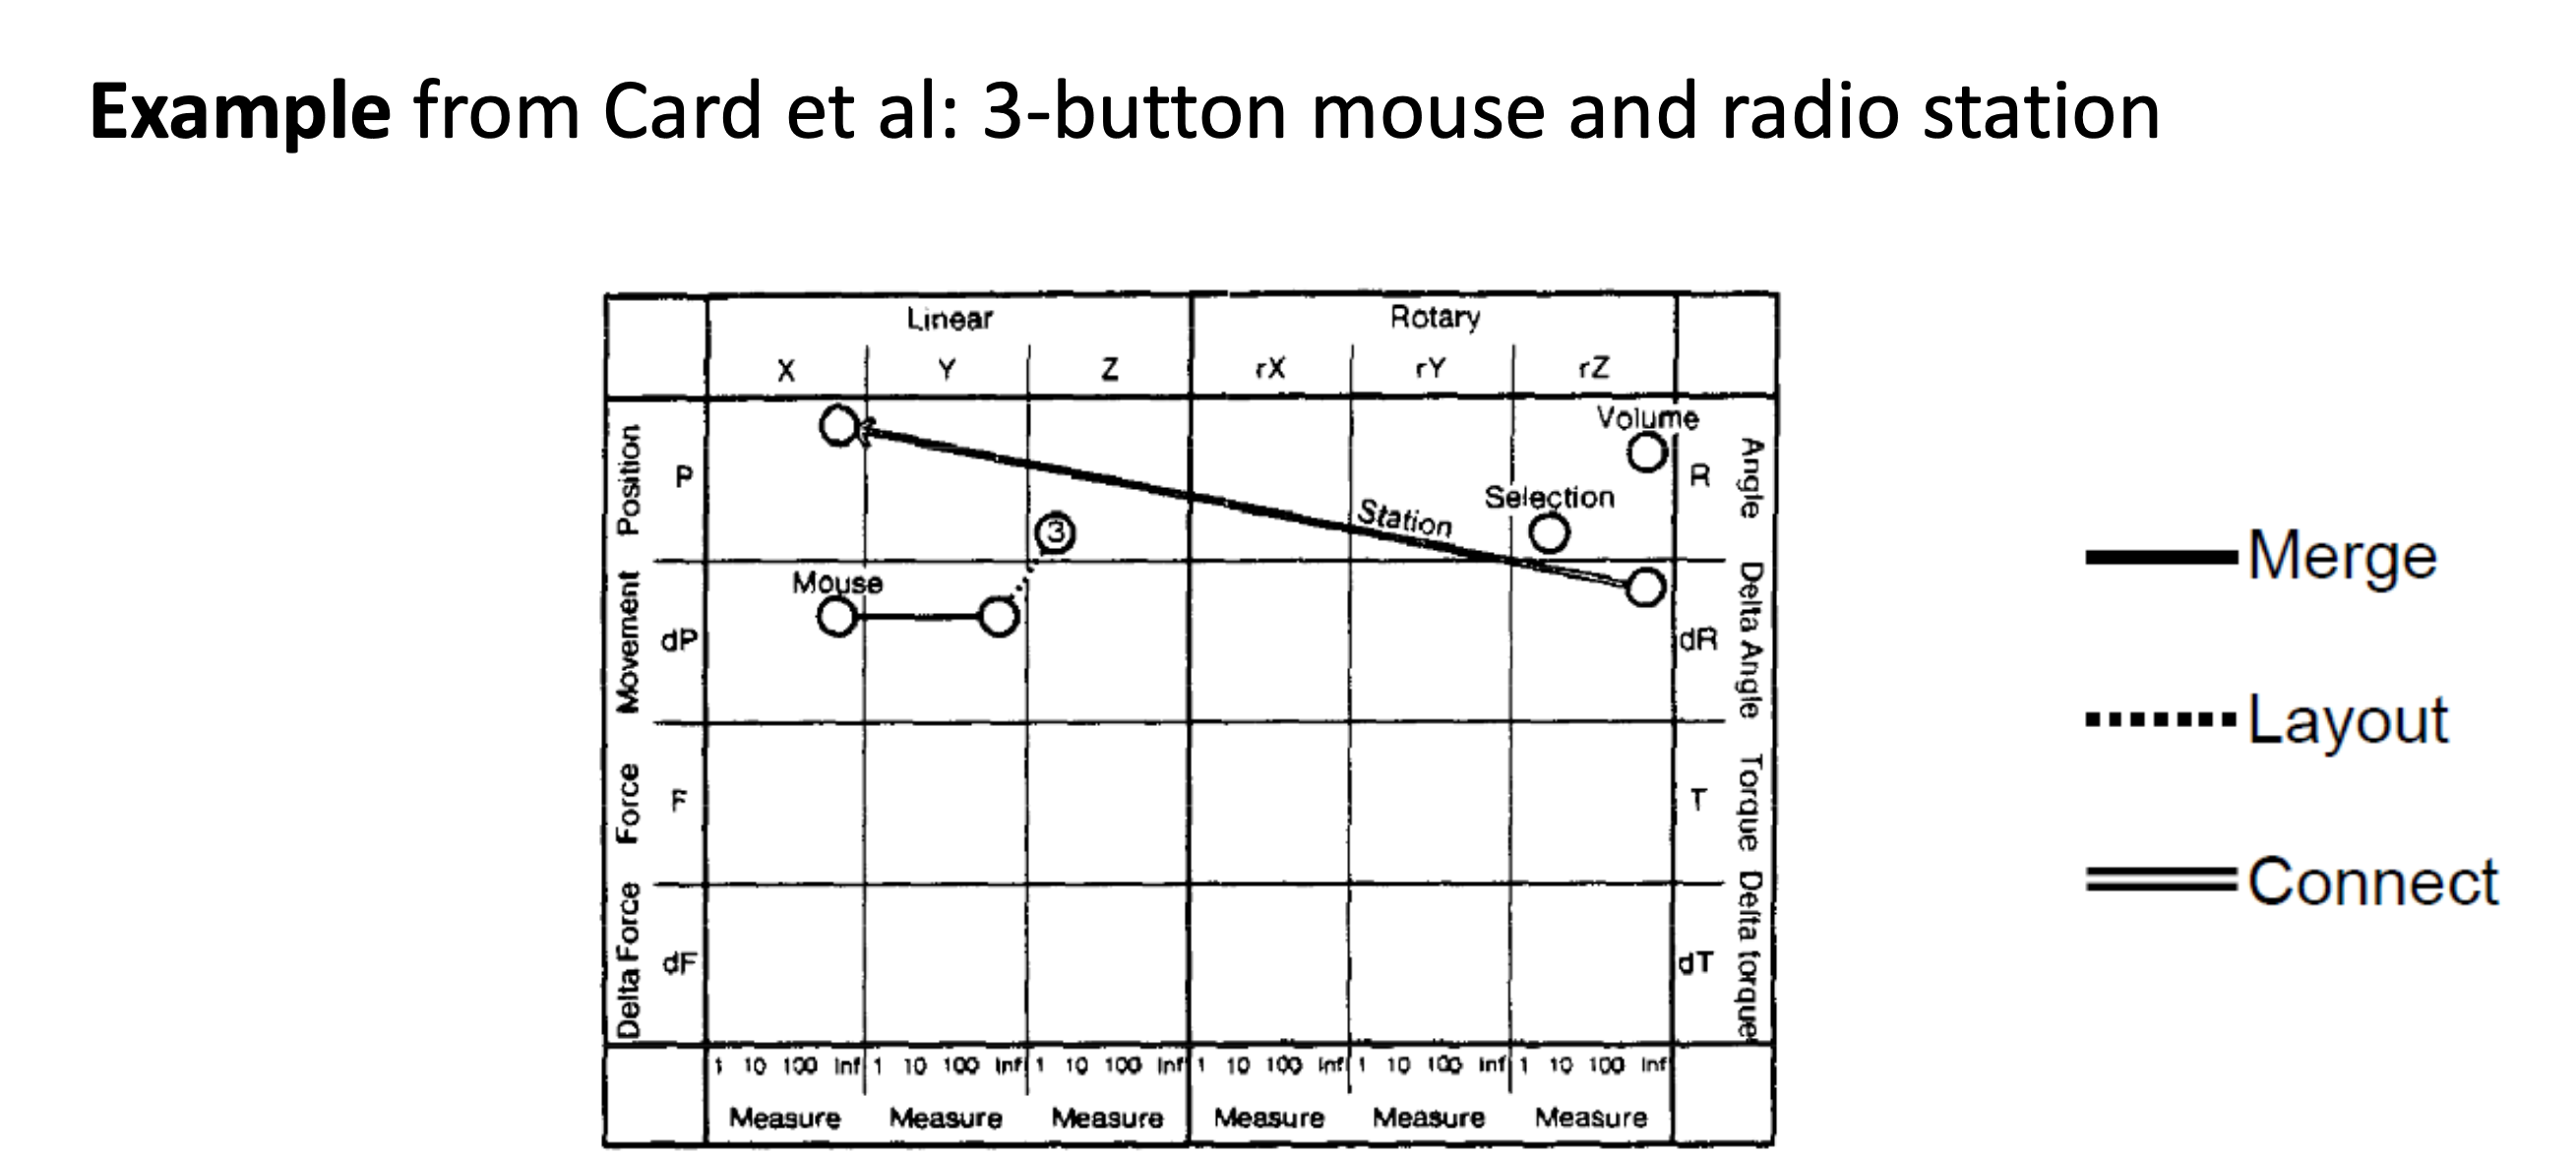
\includegraphics[width=\linewidth]{card_graphical_representation.png}
\end{center}


\textbf{Input Decoding} \smallskip

\textit{Touch Input} \smallskip

Issues with touch: It's noisy and touch area larger than the target. Also visual occlusions. Mobility increaases accuracy issues. 

\begin{center}
	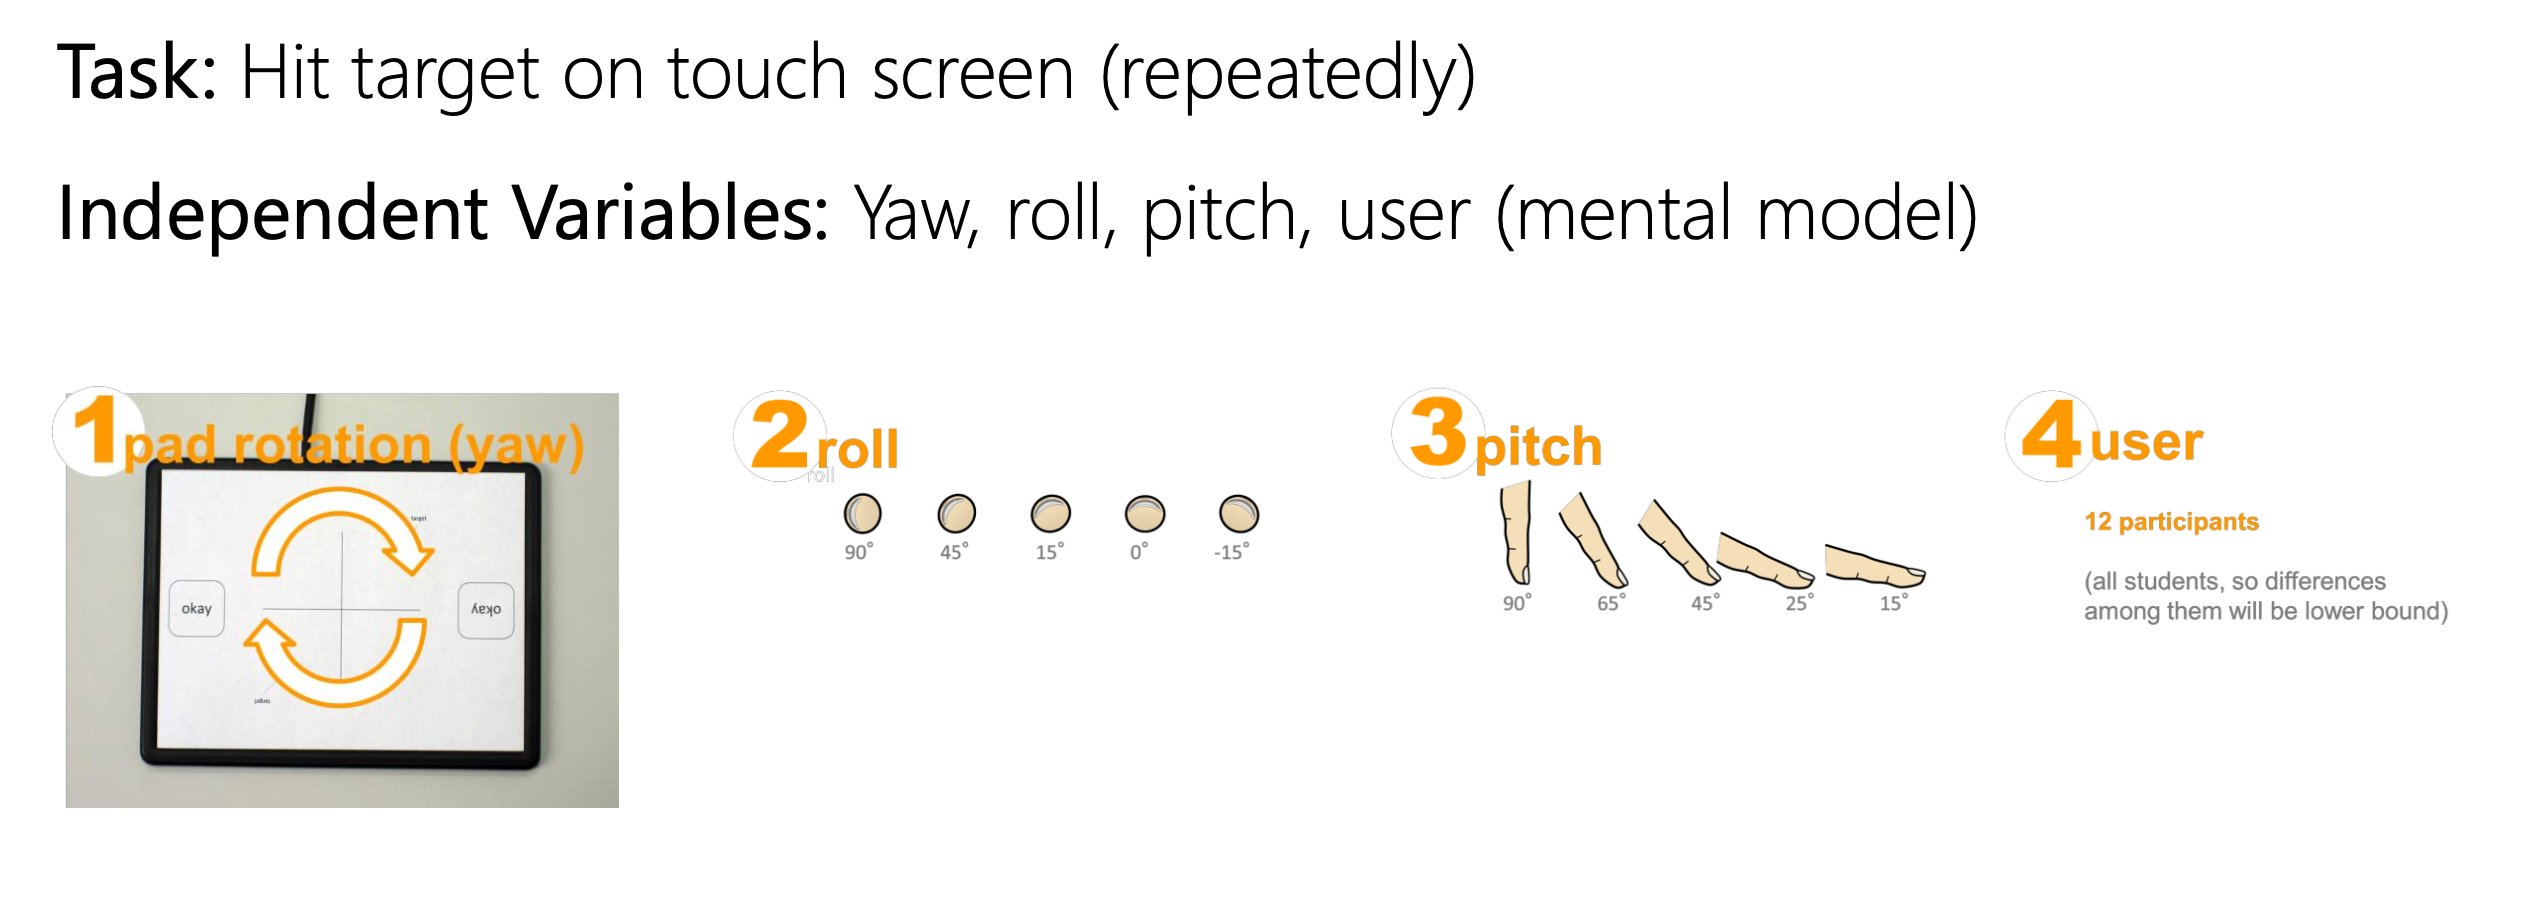
\includegraphics[width=\linewidth]{touch_experiment.png}
\end{center}

We record every trial as a dot at the touch location. Without influence of independent variables should result in circles. If the locations fall into clusters we can compensate if condition is know. \medskip

\textit{Minimum Touch Input Size}

\begin{center}
	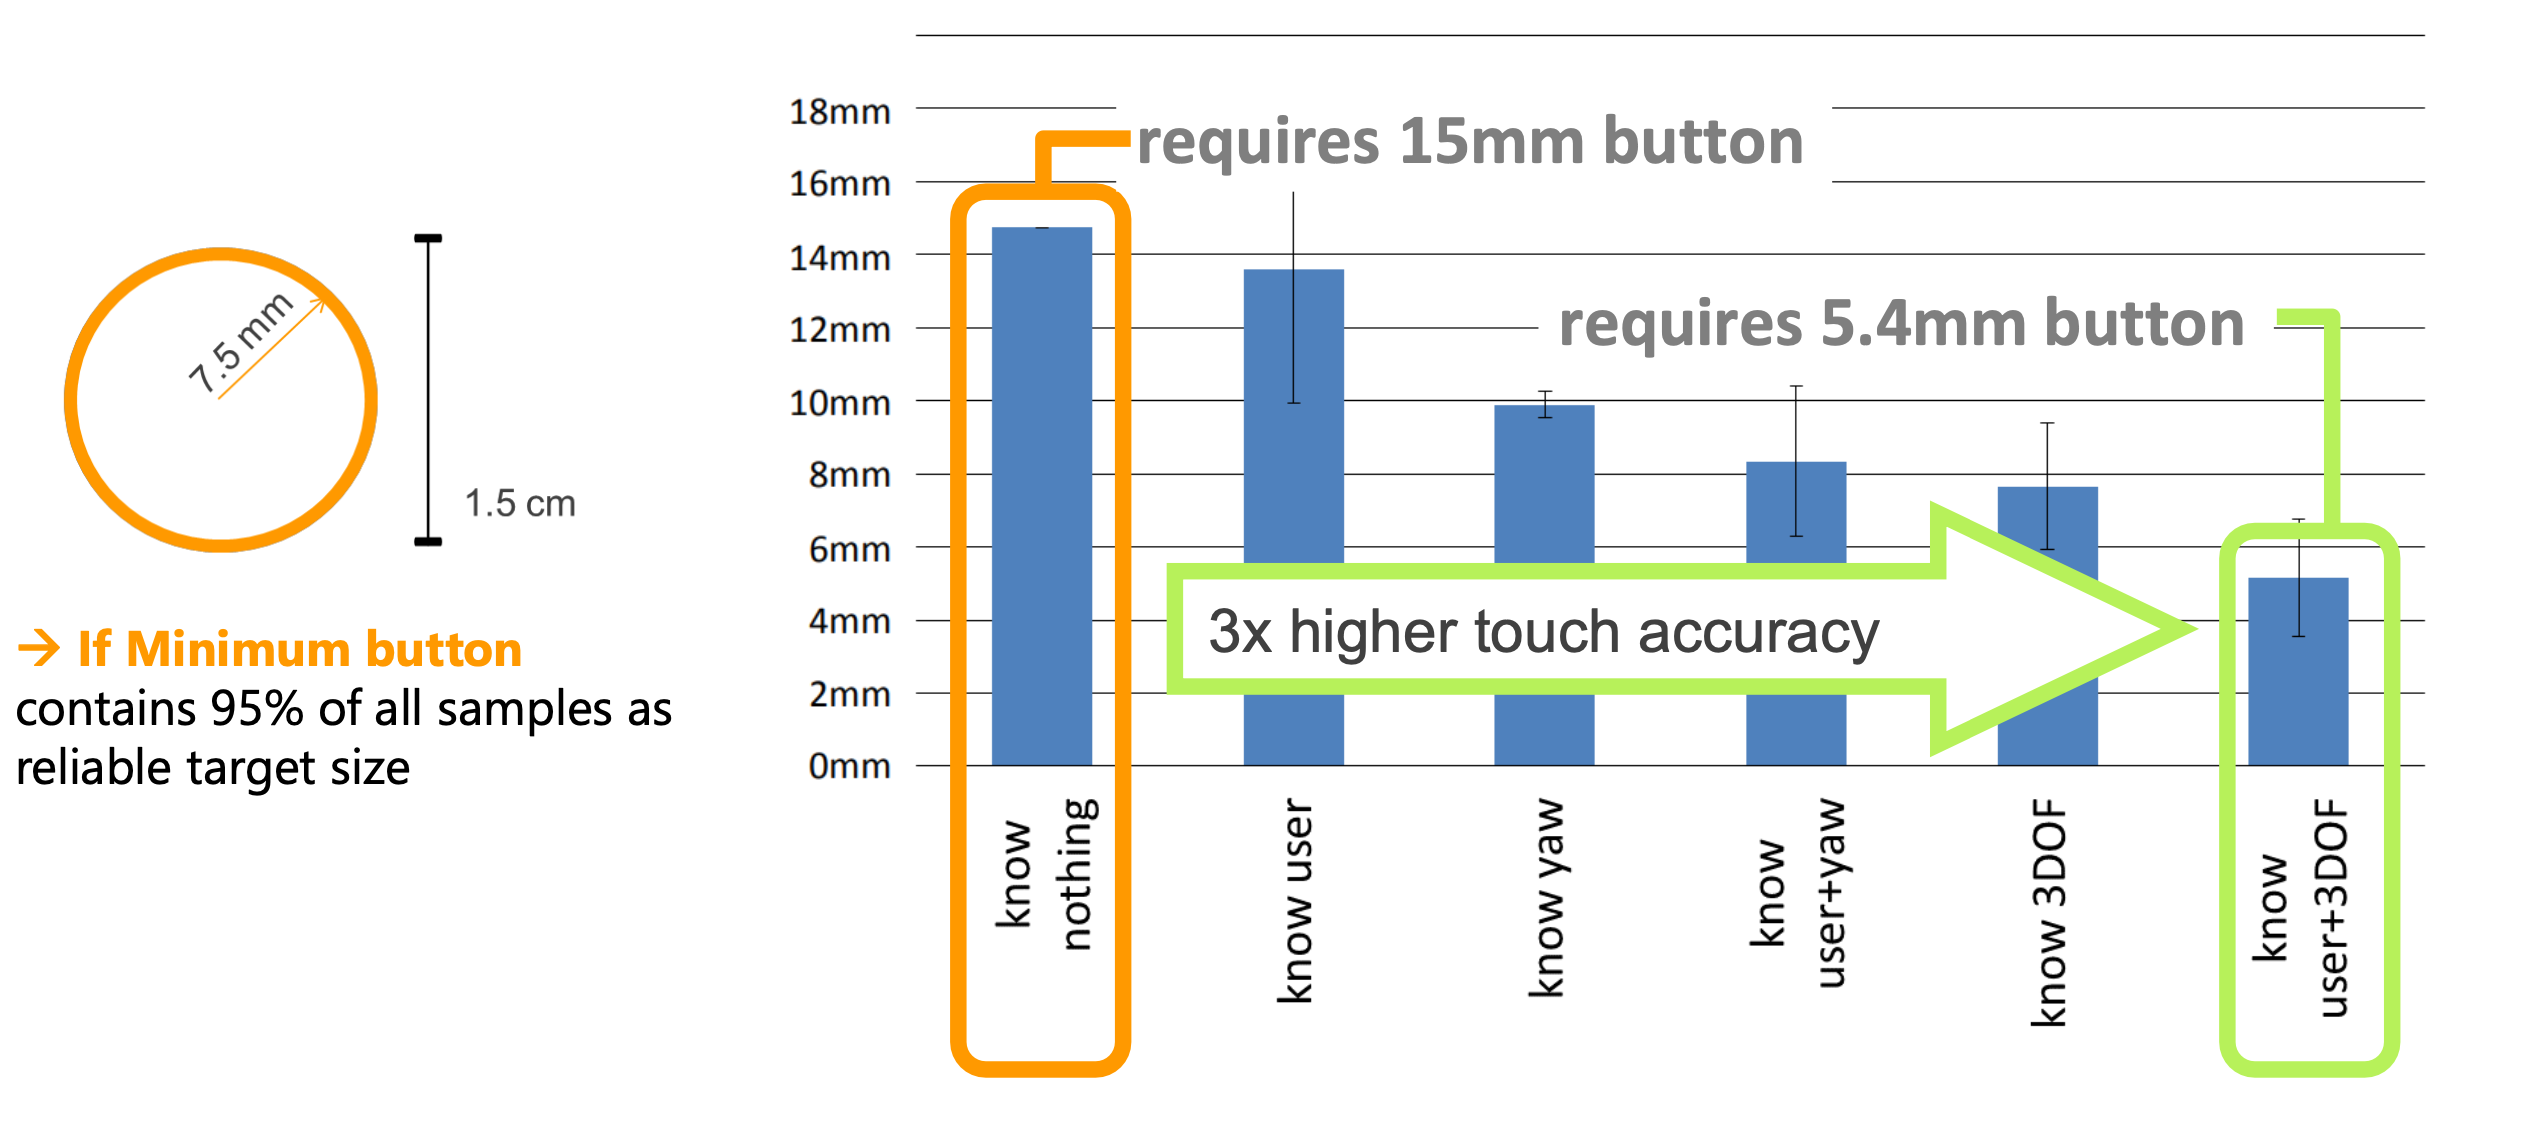
\includegraphics[width=\linewidth]{button_size.png}
\end{center}

\textit{Representing Input} \smallskip


\begin{center}
	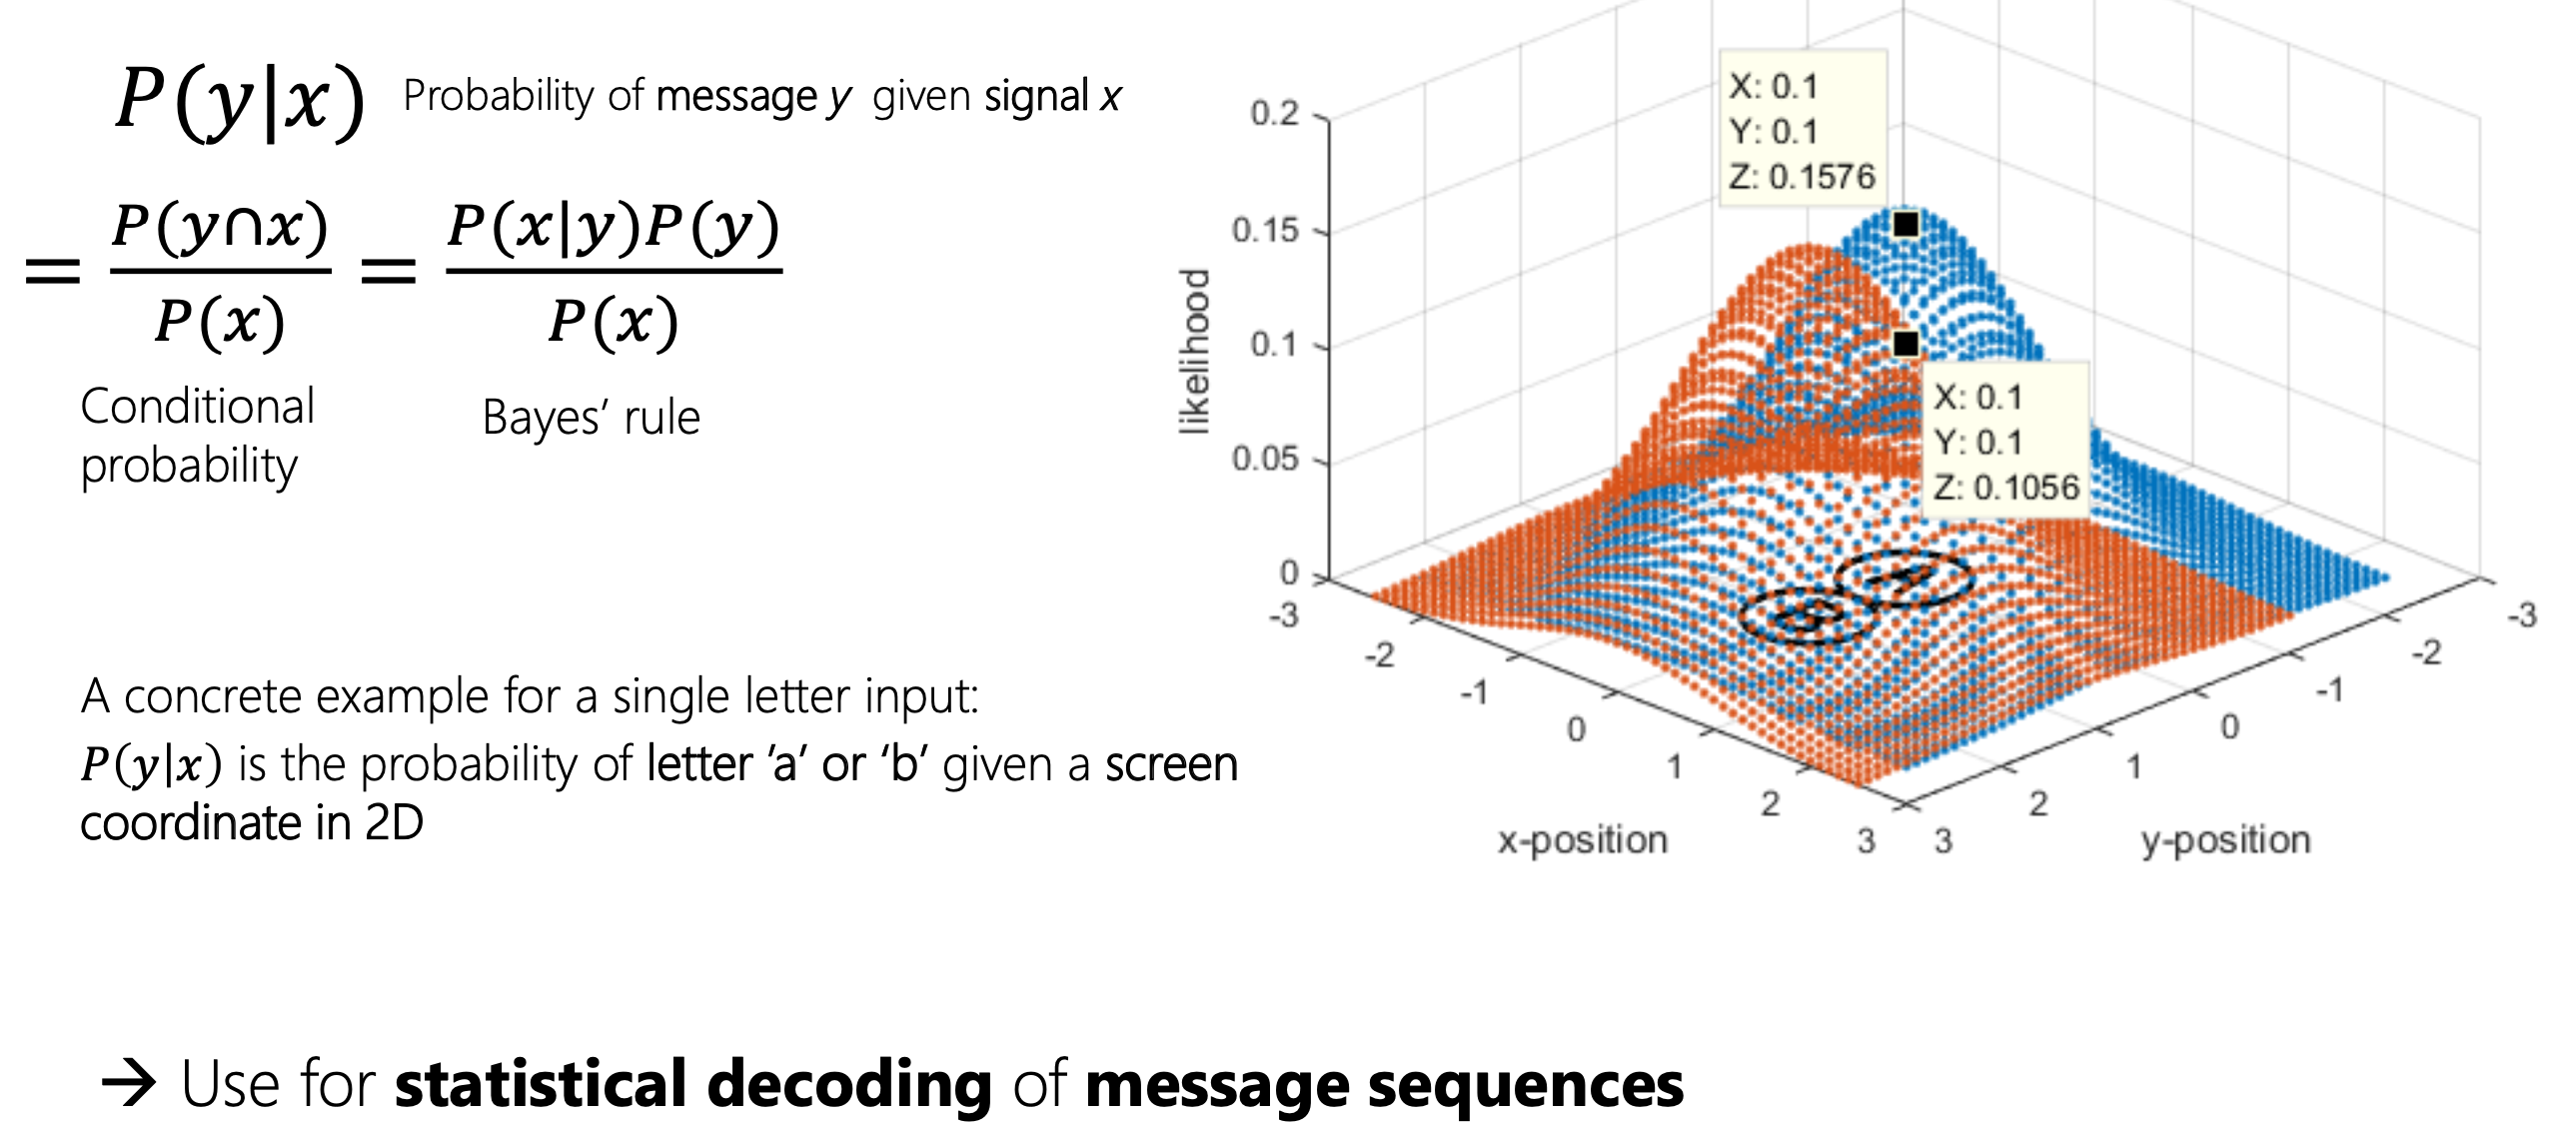
\includegraphics[width=\linewidth]{representing_input.png}
\end{center}

\textit{Sequence decoding} \smallskip

\begin{center}
	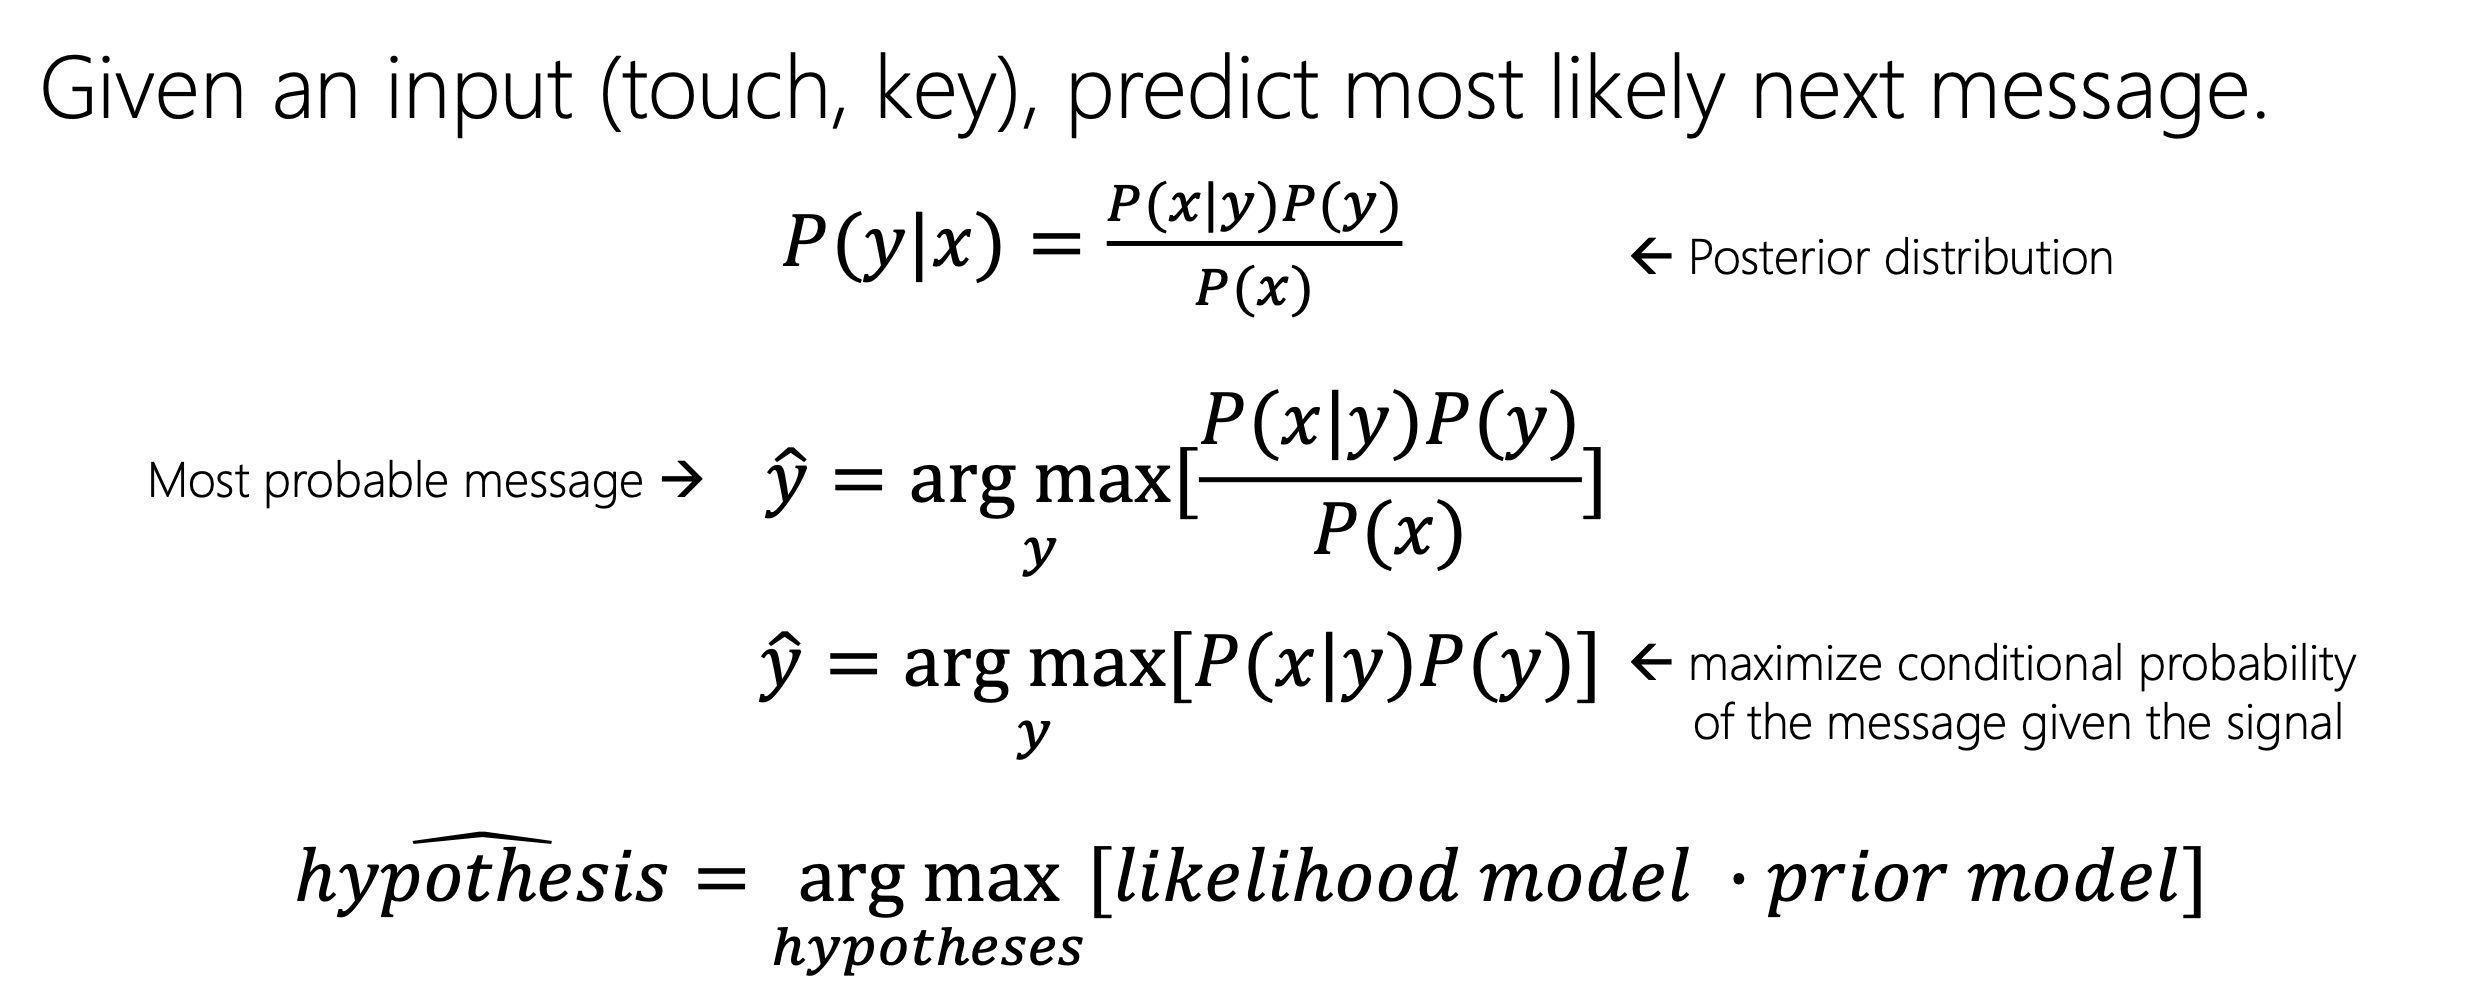
\includegraphics[width=\linewidth]{sequence_decoding.png}
\end{center}

An example would be to investigate noisy sequences of input and identify the most likely sequence of intended presses.
Observation would be the 2D screen coordinates of tap and the observation sequence are the time-ordered observations. 
\smallskip

A token in this context would be a datastructure containing the accumulated probability of hypothesis. 
$$Acc\_Prop_{n+1} = Acc\_Prob_{n} * prior * likelihood$$


\textit{Simple sequence decoding} \smallskip

One token per hypothesis per obervation. 


\begin{center}
	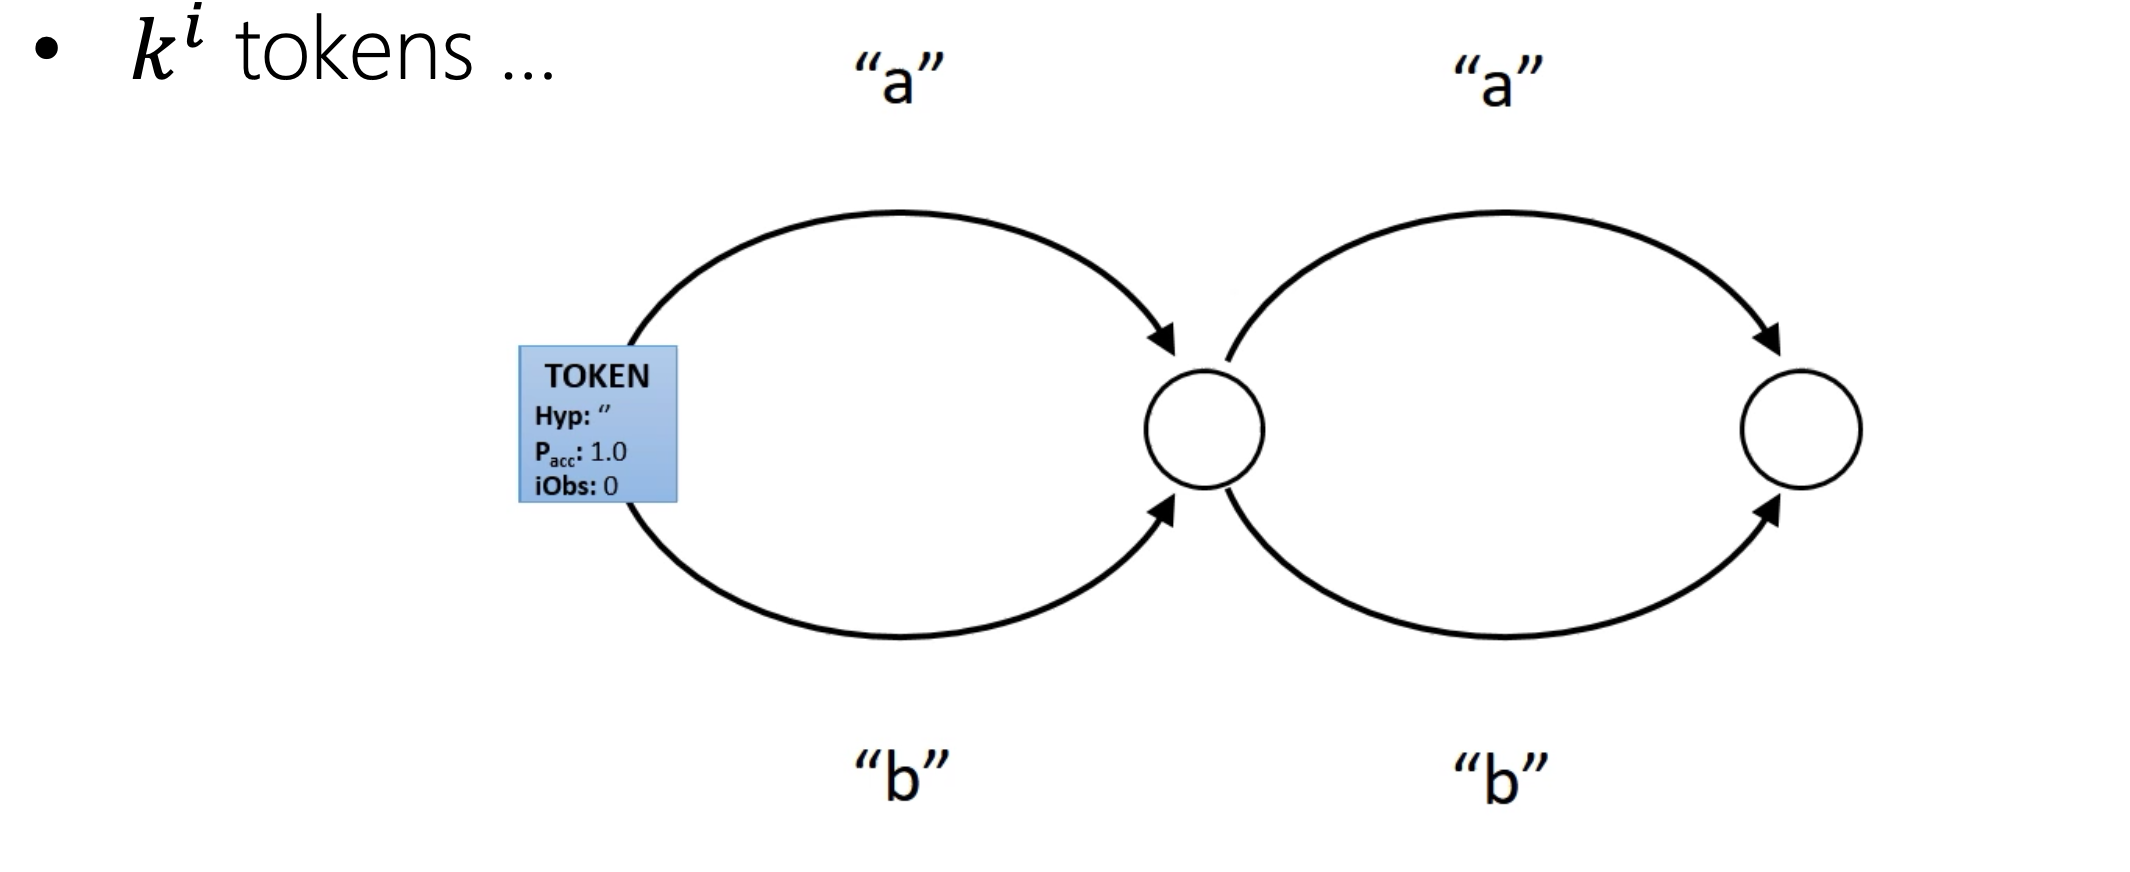
\includegraphics[width=\linewidth]{simple_sequence_decoding.png}
\end{center}


\textit{Substitution-only decoder} \smallskip

\begin{center}
	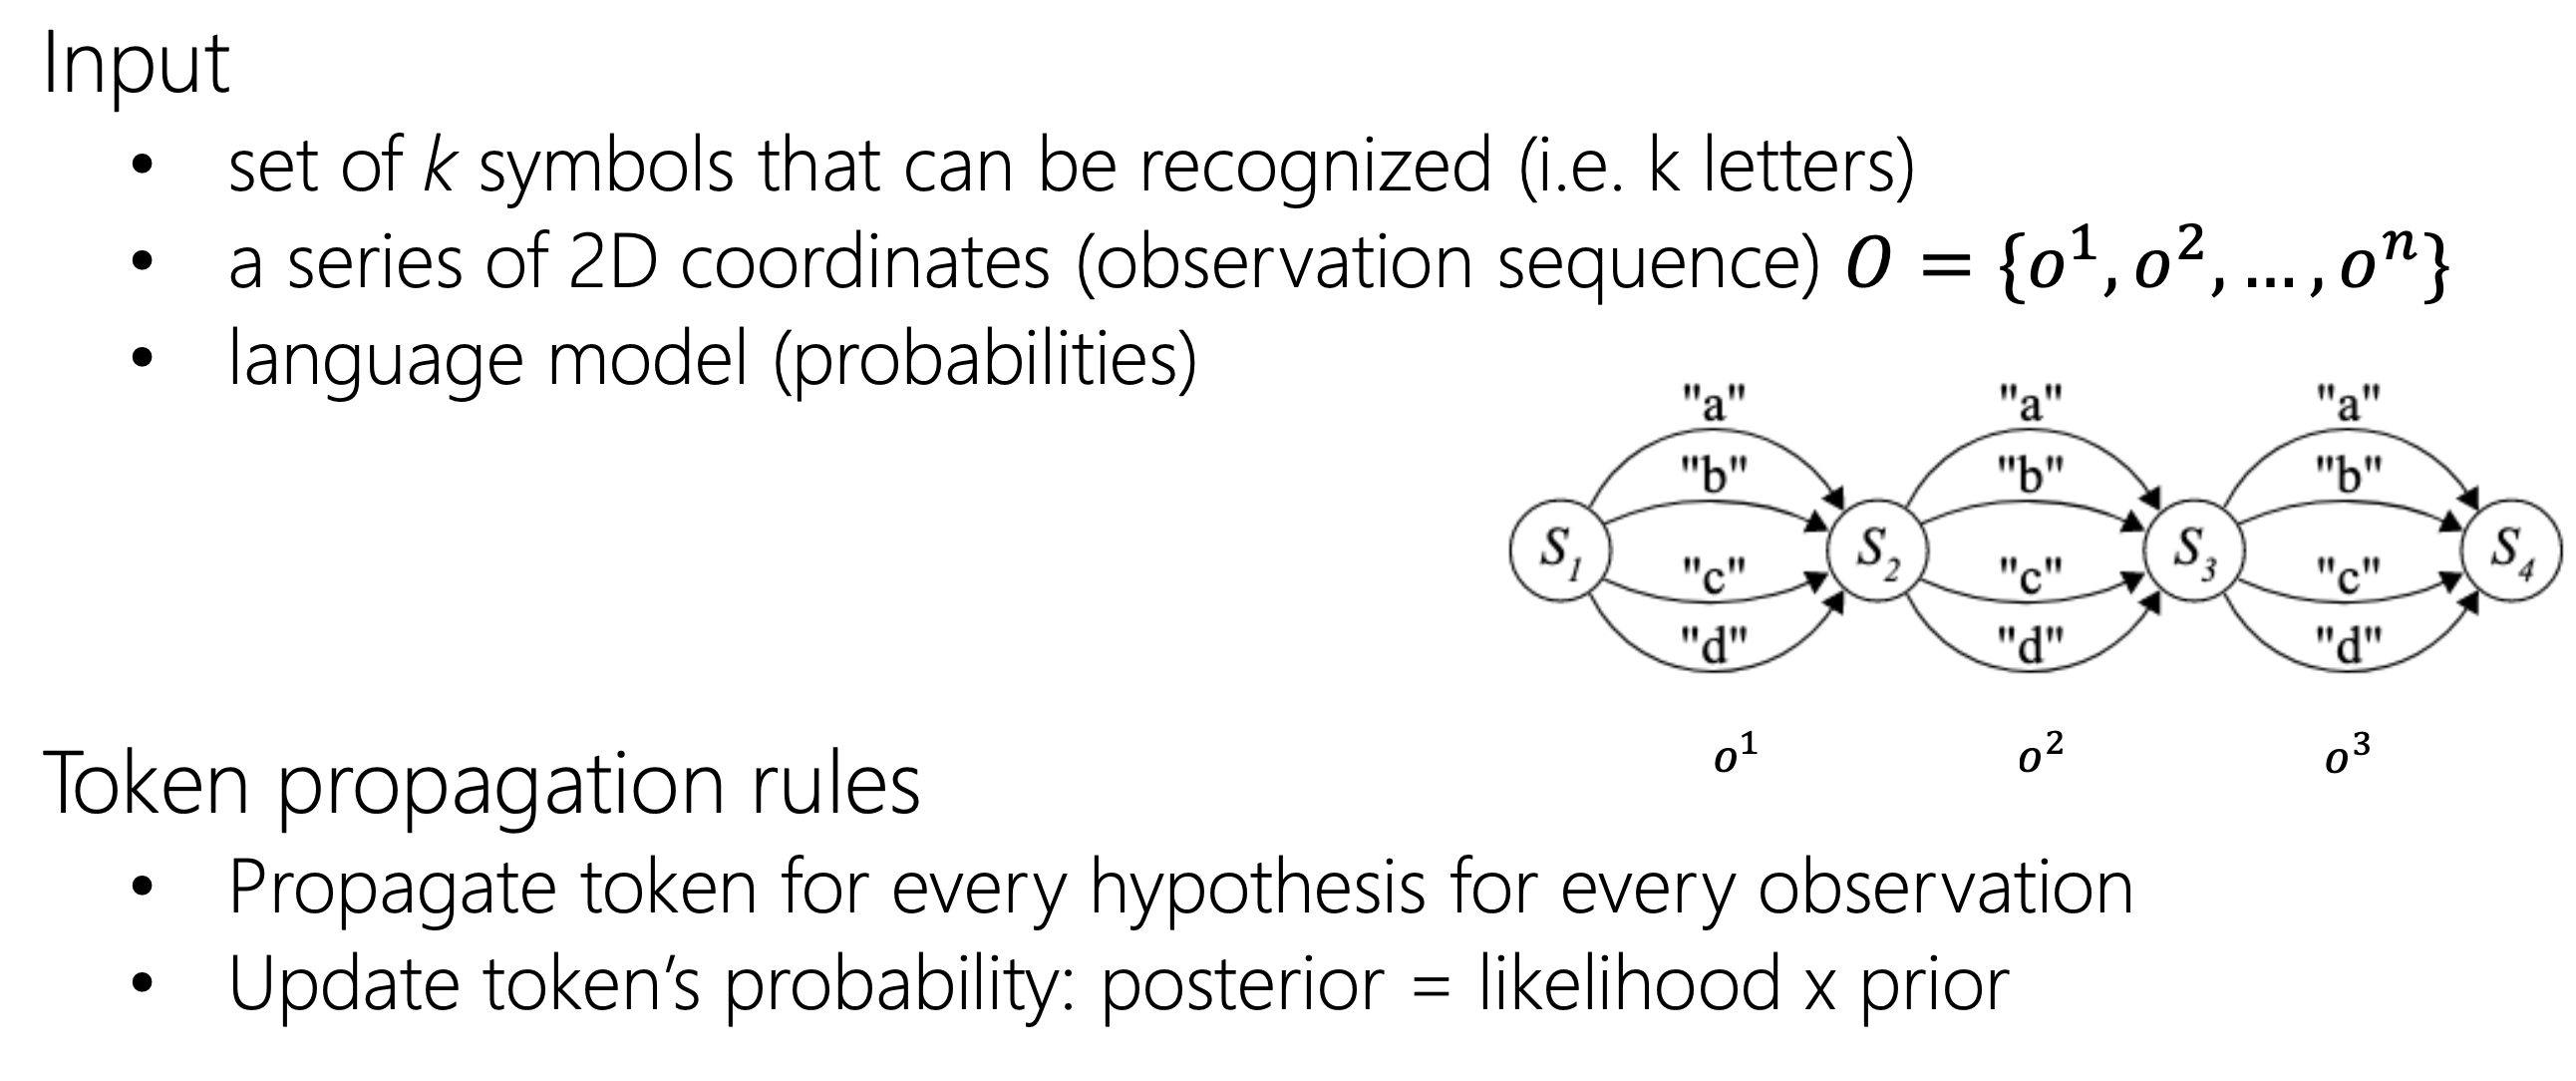
\includegraphics[width=\linewidth]{substitution_only_decoder.png}
\end{center}

\textit{Bream Pruning} \smallskip

we have an infinite search space but only a few plausible hypothesis. We prevent propagation of unlikely tokens. 

Rules of beam Pruning: 

\begin{itemize}[itemsep=-5pt, topsep=0pt, leftmargin=*]
	\item Only propagate a token if its probability is among the n-best probs for the observation so far 
	\item If the new prob of the observation is among the n-best then update the list of tokens to propagate
\end{itemize}

Threshold is also known as beam size. 

\begin{center}
	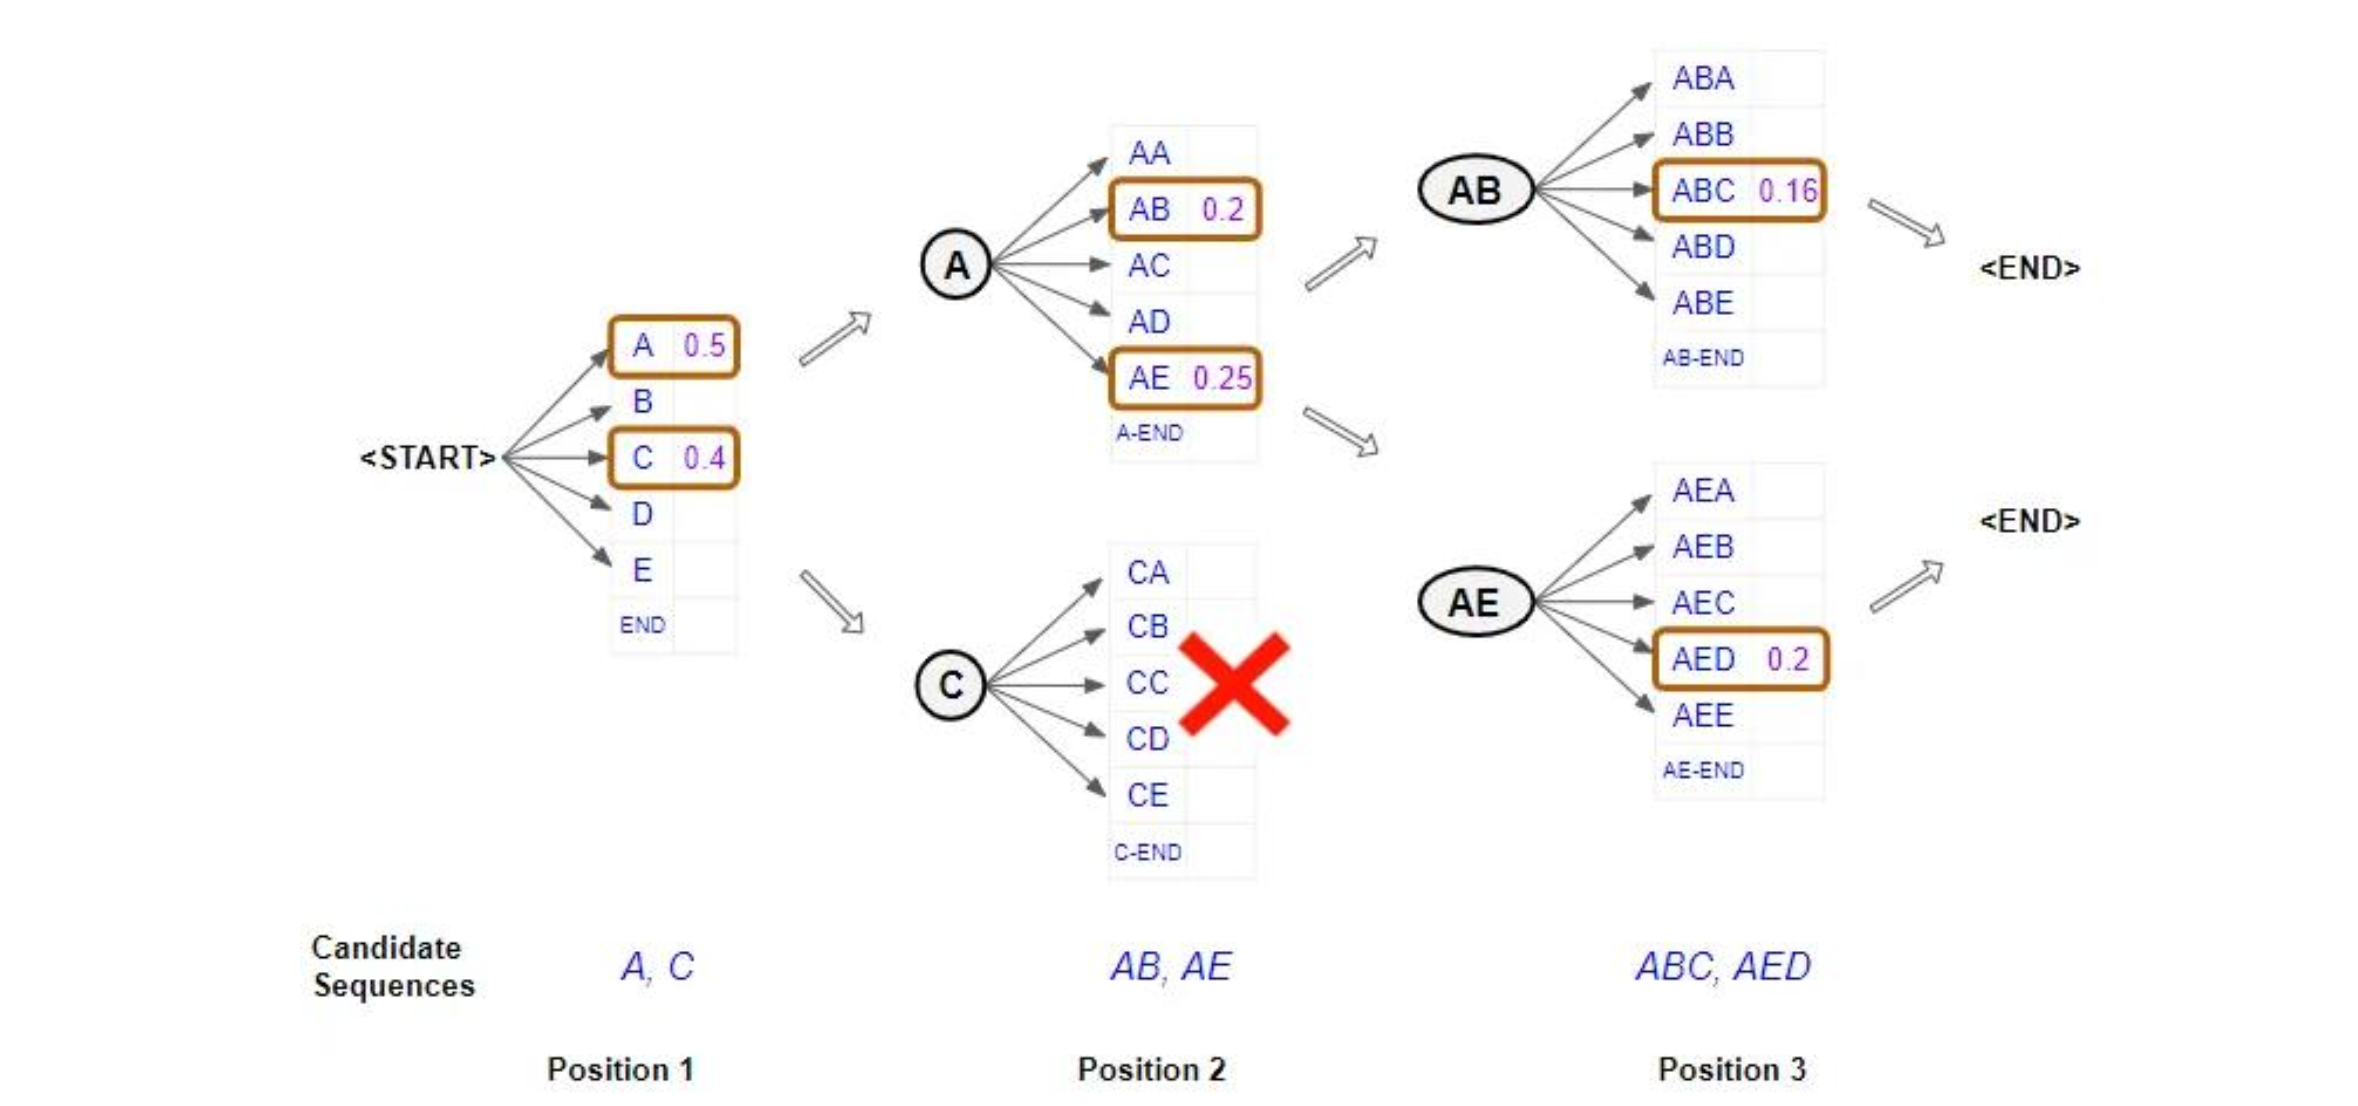
\includegraphics[width=\linewidth]{beam_pruning.png}
\end{center}

\textit{Language models} \medskip

Probabilities for the decoder come from Language models. Language models are the probability of individual words or word sequences. 
A vast amount of letter combinations is unlikely to be written. These models capture valid letter and word sequences and assign them probabilities. 
These probabilities can be leveraged to infer or predict what users want to write, based on what they have already written. \medskip

The simplest models are uni- or bigrams. (Unigram contains one token only and bigrams obviously two). \medskip

\textit{Trigram Model}

\begin{center}
	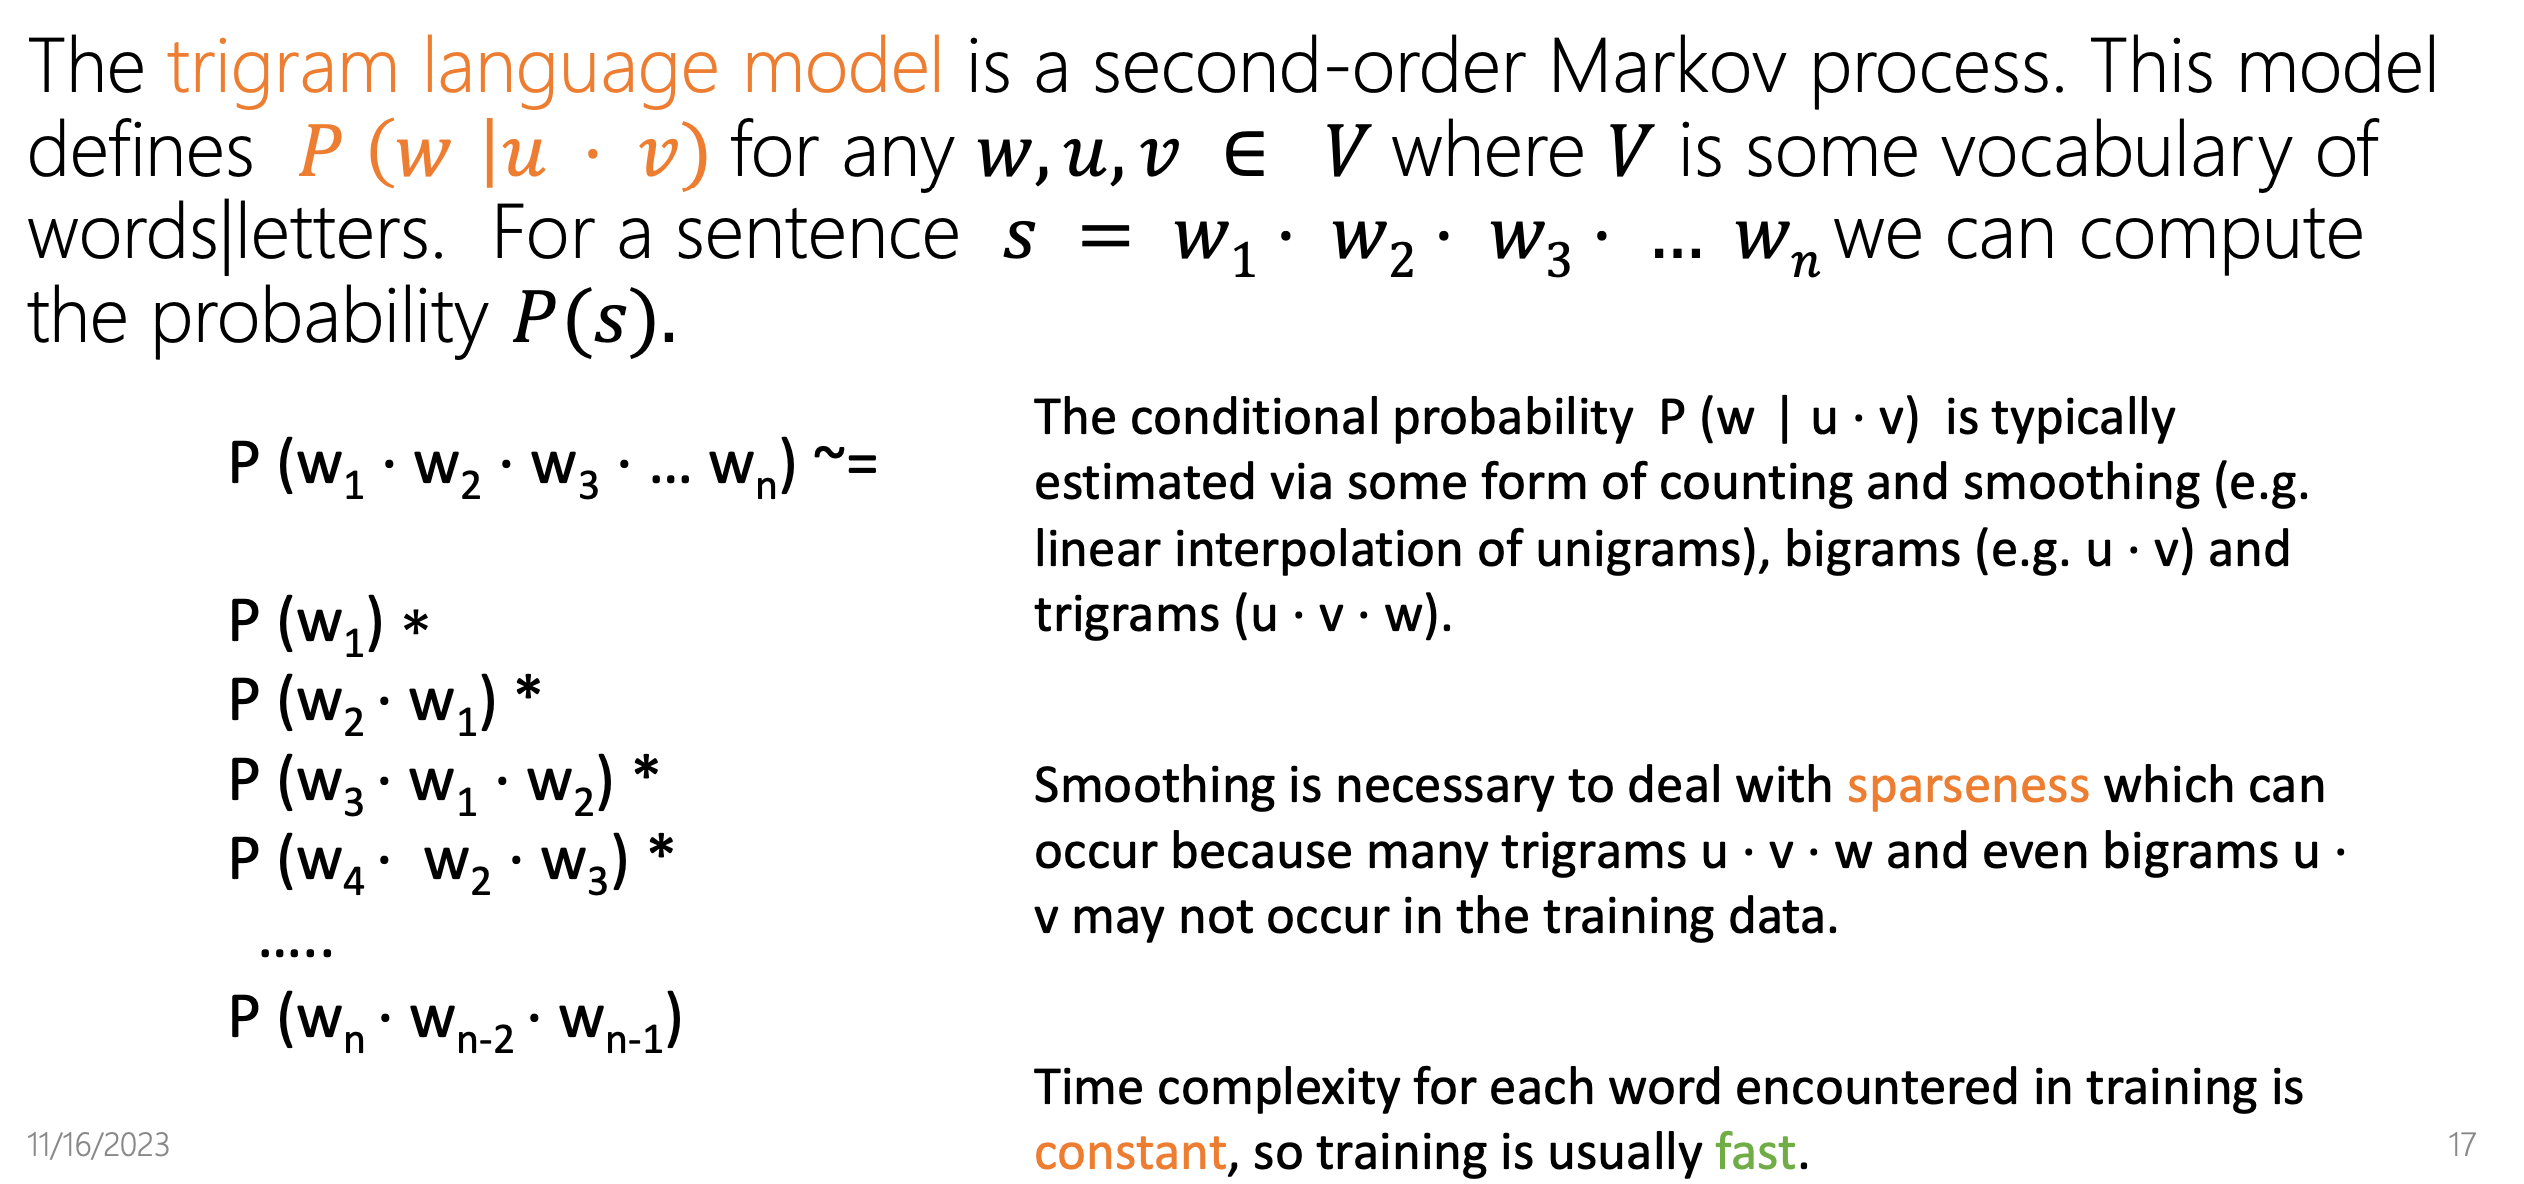
\includegraphics[width=\linewidth]{trigram_model.png}
\end{center}

\textit{Trigram Model Example}

\begin{center}
	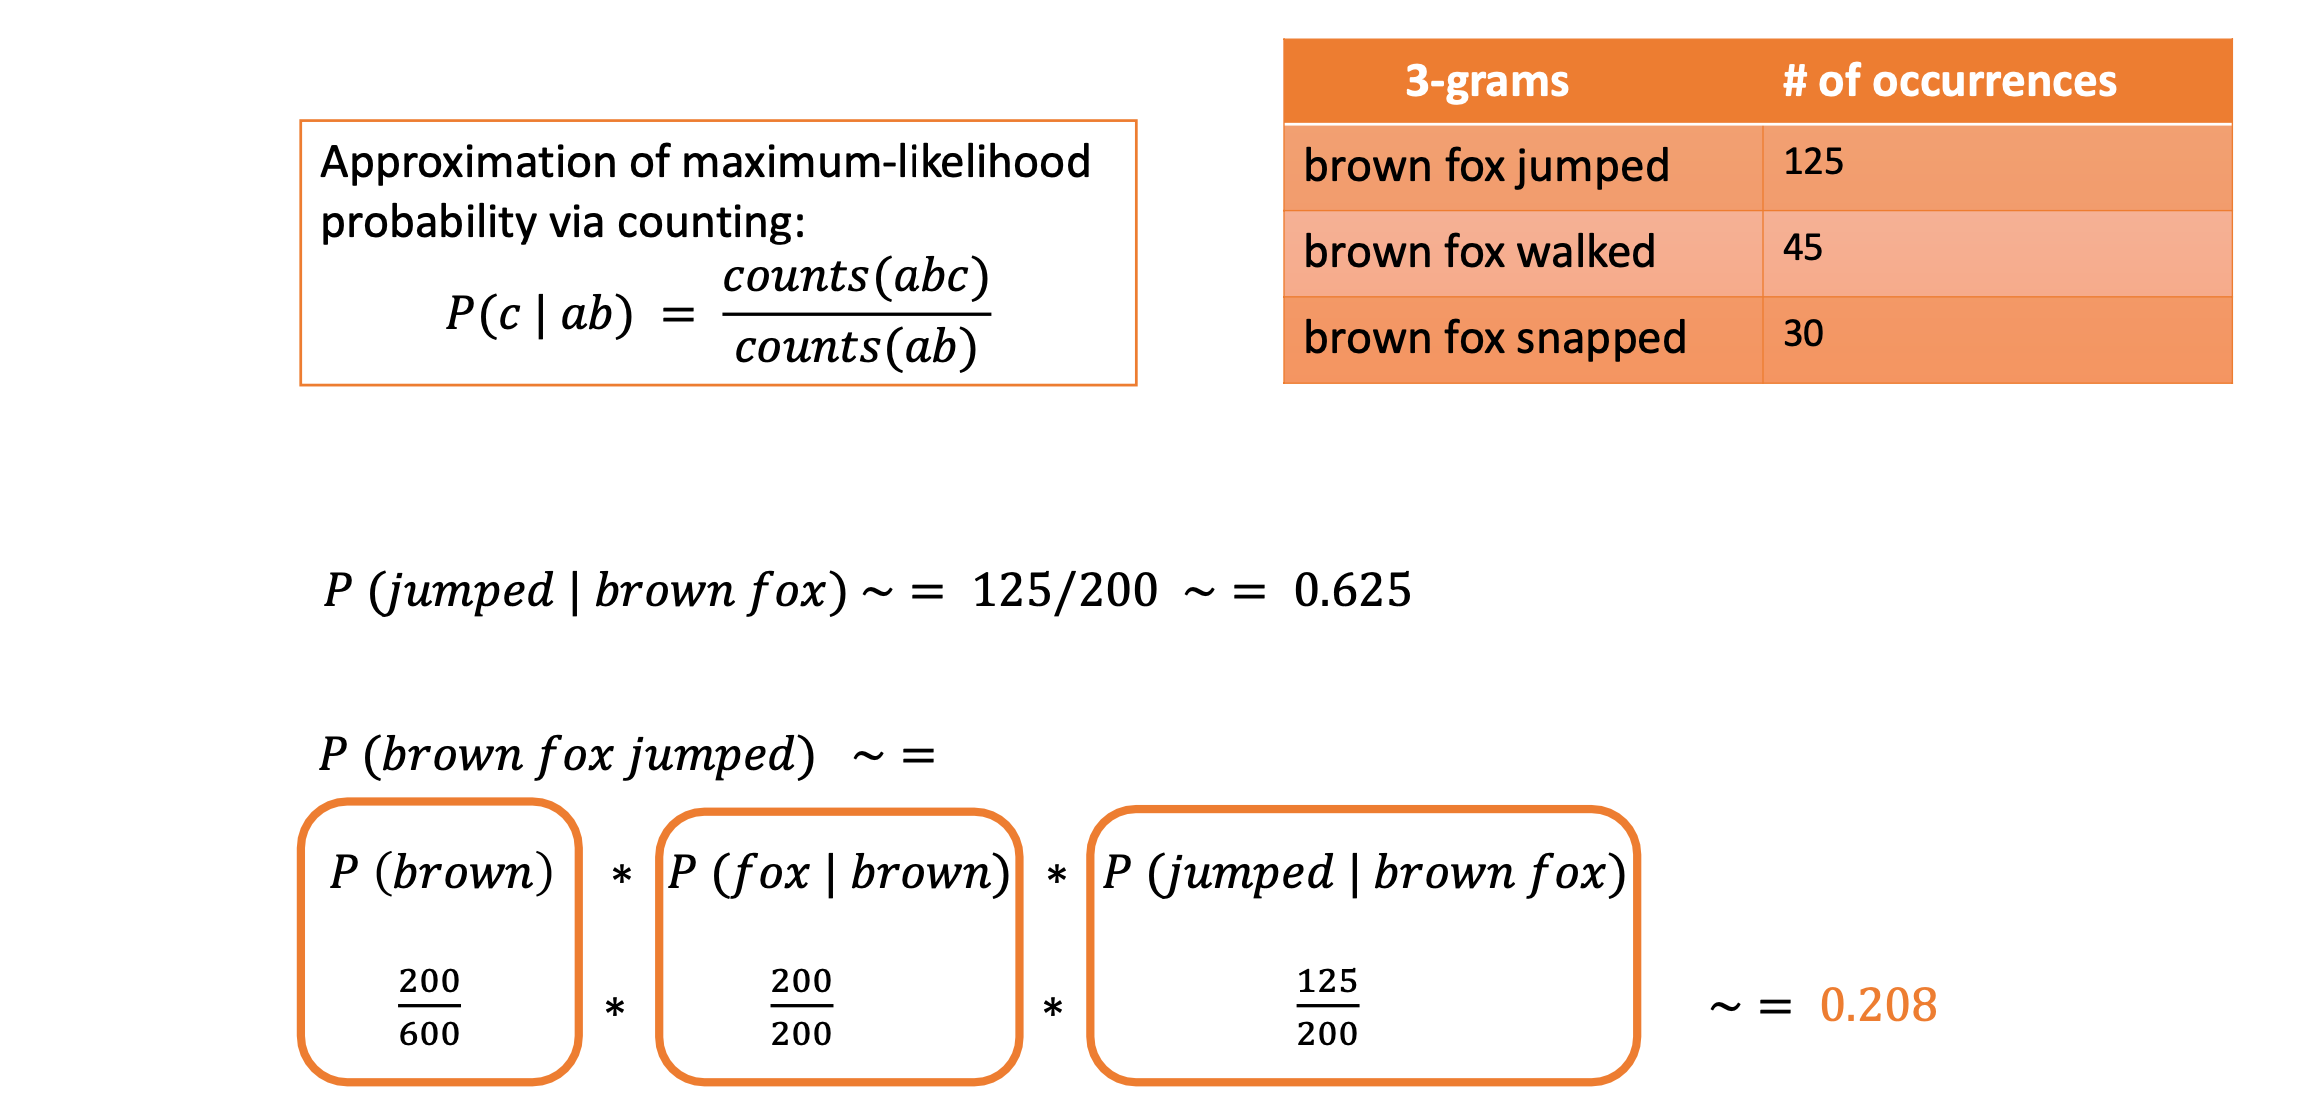
\includegraphics[width=\linewidth]{trigram_model_example.png}
\end{center}

\textit{Advanced statistial language models} \smallskip

Recurrent neural network (RNN) and Generative Pre-trained Transformers(GPT) are able to capture more complex relationsships for many to many token mappings. 

\medskip

We can then combine probabilities from the touch model with a language model to get the most likely key for a touch. 


\begin{center}
	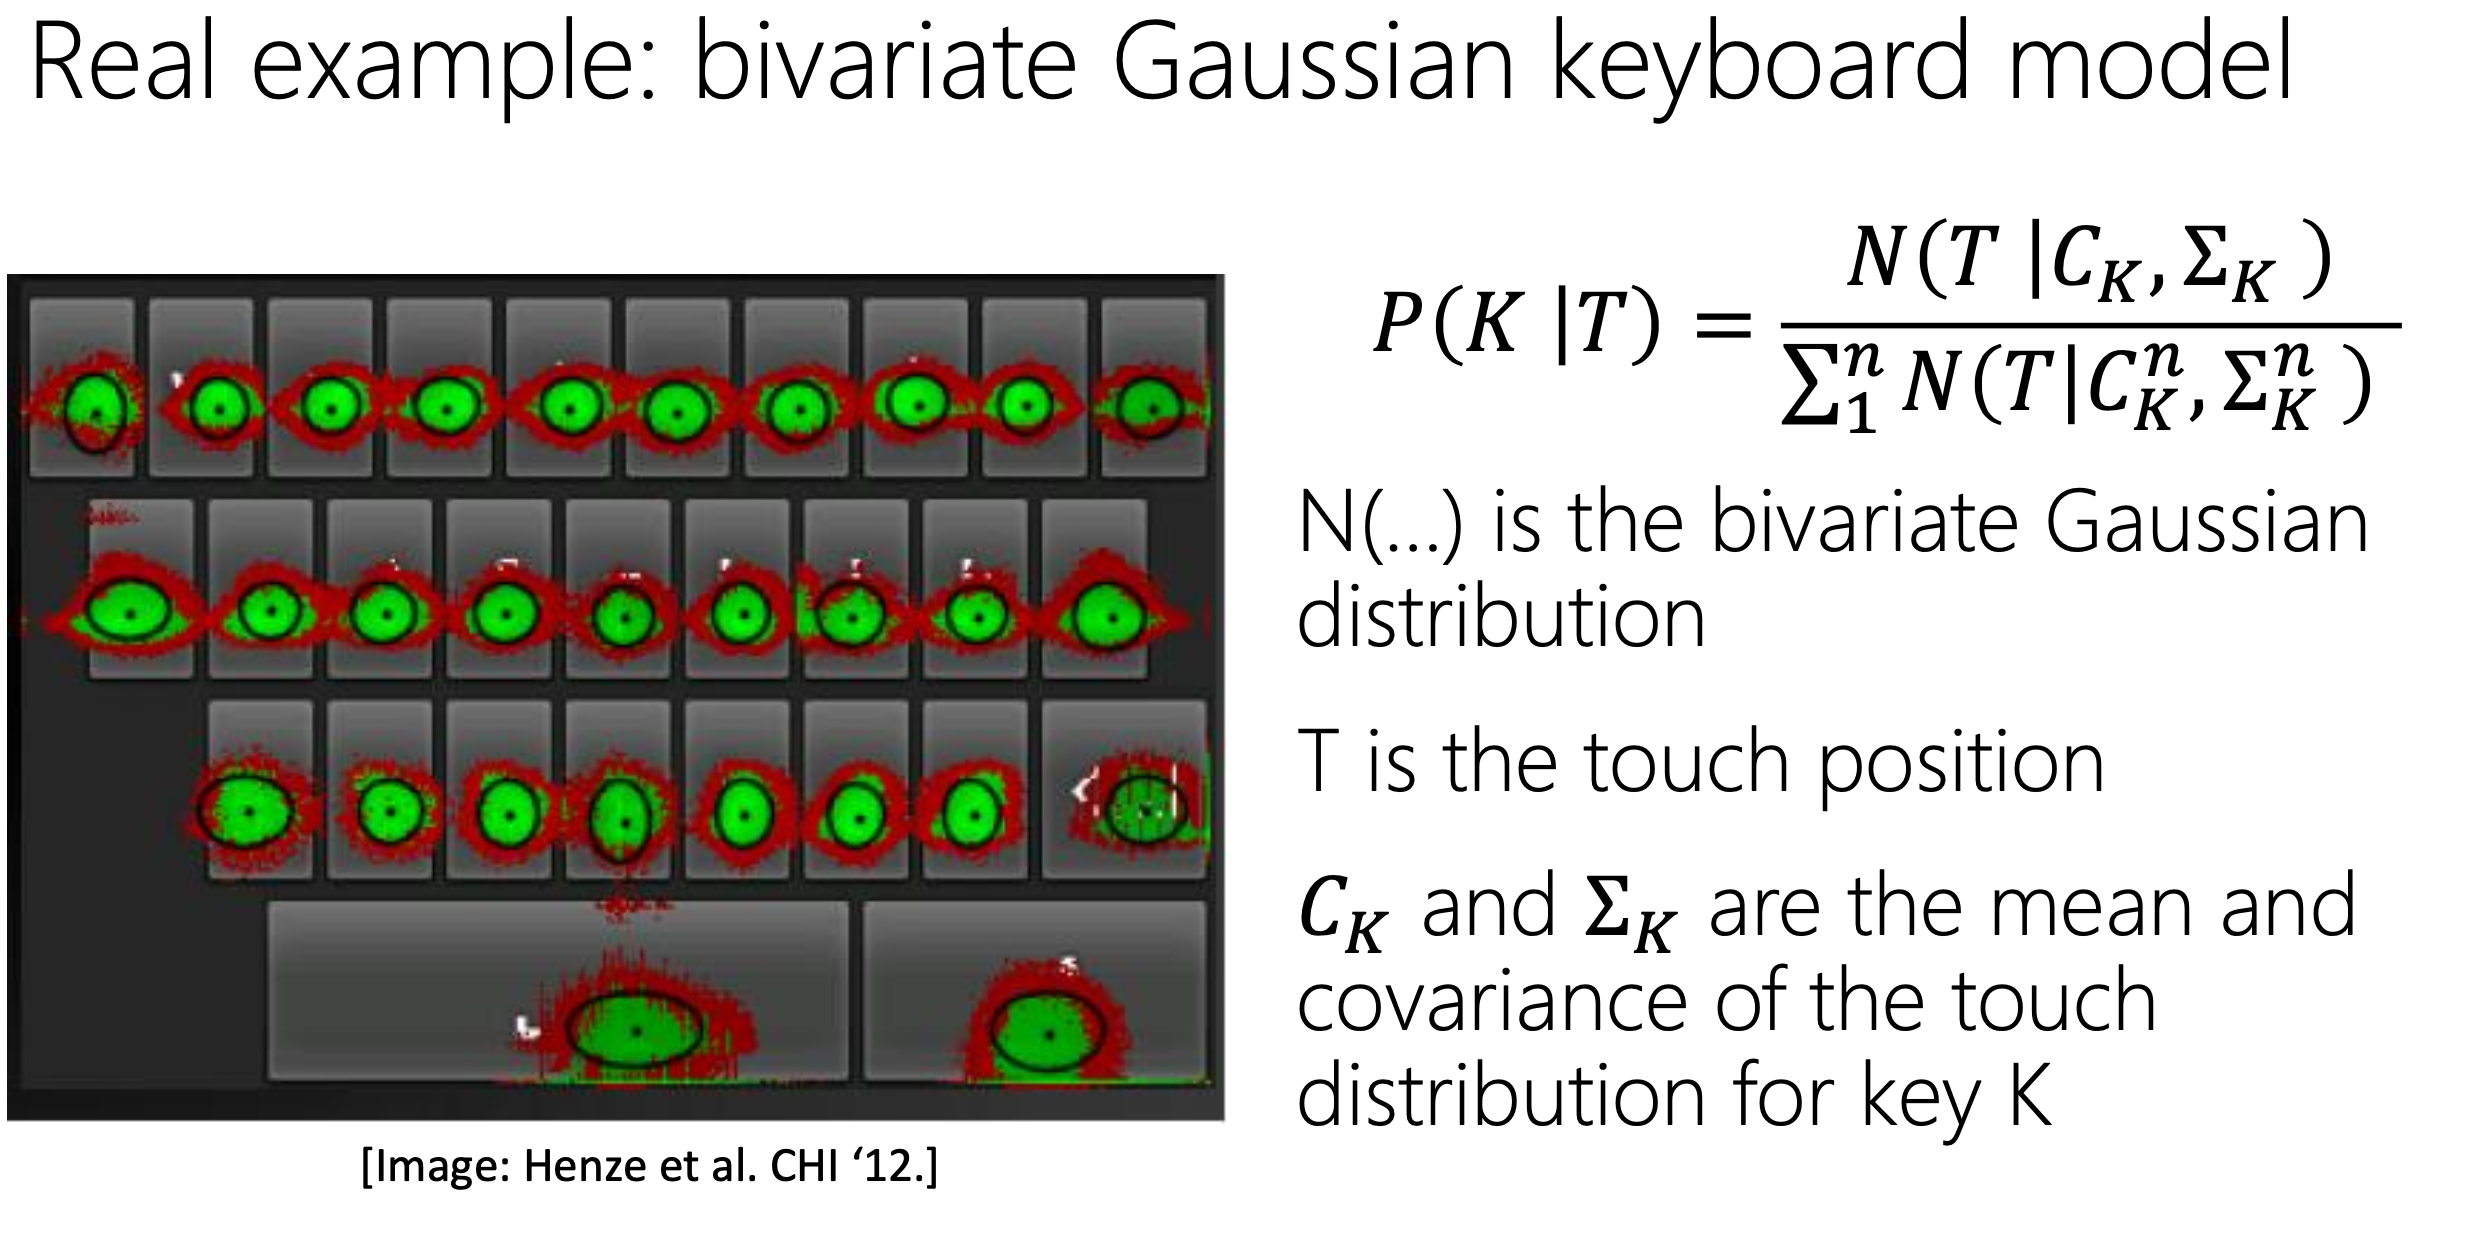
\includegraphics[width=\linewidth]{bivariate_gaussian_keyboard.png}
\end{center}

\textit{Application Examples} \smallskip

\begin{itemize}[itemsep=-5pt, topsep=0pt, leftmargin=*]
	\item Predictive text input
	\item Text input beyond screens
	\item Accessible mixed reality
\end{itemize}

(Check slides if you want to see more on these).
